\documentclass[utf8]{frontiersSCNS} % for Science, Engineering and Humanities
\usepackage{url,hyperref,lineno,microtype,subcaption}
\usepackage[onehalfspacing]{setspace}

\linenumbers

%%% BEGIN added by AJS
\usepackage{xltxtra} % also loads 'fontspec'
\defaultfontfeatures{Ligatures=TeX}
\setmainfont{Minion Pro}
\setsansfont[Scale=MatchLowercase]{Myriad Pro}
\setmonofont[Scale=MatchLowercase]{Ubuntu Mono}
% \setmathfont{Minion Math}

\frenchspacing
\usepackage{textgreek}
\usepackage{ragged2e}  % for '\RaggedRight' macro (allows hyphenation)
\usepackage{booktabs} % nice tables without vertical lines
\setlength\heavyrulewidth{0.1em}
\setlength\lightrulewidth{0.0625em}
\usepackage{siunitx}
    \sisetup{%
        detect-mode,
        group-digits            = false,
        input-symbols           = ( ) [ ] - + < > * §,
        table-align-text-post   = false,
        round-mode              = places,
        round-precision         = 3
        }

        % SECTION, SUBSECETC.TITLES
        \usepackage[compact]{titlesec}
        \titleformat{\chapter}
          {\normalfont\LARGE\sffamily\bfseries}
          {\thechapter}
          {1em}
          {}
        \titleformat{\section}
          {\normalfont\LARGE\sffamily\bfseries}
          {\thesection}
          {1em}
          {}
        \titleformat{\subsection}
          {\normalfont\Large\sffamily\bfseries}
          {\thesubsection}
          {1em}
          {}
        \titleformat{\subsubsection}
          {\normalfont\large\sffamily\bfseries\slshape}
          {\thesubsubsection}
          {1em}
          {}
        % \titlespacing*{<command>}{<left>}{<before-sep>}{<after-sep>}
        \titlespacing*{\chapter}
          {0pt}
          {1.2ex plus 1ex minus .2ex}
          {0.5ex plus .1ex minus .1ex}
        \titlespacing*{\section}
          {0pt}
          {1.2ex plus 1ex minus .2ex}
          {0.5ex plus .1ex minus .1ex}
        \titlespacing*{\subsection}
          {0pt}
          {1.2ex plus 1ex minus .2ex}
          {0.5ex plus .1ex minus .1ex}
        \titlespacing*{\subsubsection}
          {0pt}
          {1.2ex plus 1ex minus .2ex}
          {0.5ex plus .1ex minus .1ex}
 %%% END added by AJS

% Leave a blank line between paragraphs instead of using \\

\def\keyFont{\fontsize{8}{11}\helveticabold }
\def\firstAuthorLast{Smit {et~al.}} %use et al only if is more than 1 author
\def\Authors{Albertus J. Smit\,$^{1,*}$, John J. Bolton\,$^{2}$ and Robert J. Anderson\,$^{2,3}$}
% Affiliations should be keyed to the author's name with superscript numbers and be listed as follows: Laboratory, Institute, Department, Organization, City, State abbreviation (USA, Canada, Australia), and Country (without detailed address information such as city zip codes or street names).
% If one of the authors has a change of address, list the new address below the correspondence details using a superscript symbol and use the same symbol to indicate the author in the author list.
\def\Address{$^{1}$Department of Biodiversity and Conservation Biology, University of the Western Cape, Private Bag X17, Bellville 7535, South Africa \\
$^{2}$Biological Sciences Department and Marine Research Institute, University of Cape Town, Rondebosch, 7701, South Africa \\
$^{3}$Seaweed Unit, Fisheries Branch, Department of Agriculture, Forestry and Fisheries, Roggebaai, 8012, South Africa  }
% The Corresponding Author should be marked with an asterisk
% Provide the exact contact address (this time including street name and city zip code) and email of the corresponding author
\def\corrAuthor{Albertus J. Smit}

\def\corrEmail{ajsmit@uwc.ac.za}

\begin{document}
\onecolumn
\firstpage{1}

\title[Seaweeds in Two Oceans]{Seaweeds in Two Oceans: Beta-diversity}

\author[\firstAuthorLast ]{\Authors} %This field will be automatically populated
\address{} %This field will be automatically populated
\correspondance{} %This field will be automatically populated

\extraAuth{}% If there are more than 1 corresponding author, comment this line and uncomment the next one.
%\extraAuth{corresponding Author2 \\ Laboratory X2, Institute X2, Department X2, Organization X2, Street X2, City X2 , State XX2 (only USA, Canada and Australia), Zip Code2, X2 Country X2, email2@uni2.edu}


\maketitle


\begin{abstract}

%%% Leave the Abstract empty if your article does not require one, please see the Summary Table for full details.
\section{}
Several species assembly mechanisms have been proposed to structure ecological communities. We assess the biogeography of seaweeds along 2,900 km of South Africa's coastline in relation to a thermal gradient produced by the Agulhas Current, and contrast this with the environmental structure created by the Benguela Current. We subdivided the coastline into `bioregions' to examine the regional patterning. To investigate the assembly mechanisms, we decomposed Sørensen's \textbeta-diversity into `turnover' (\textbeta$_{\text{sim}}$) and `nestedness-resultant' (\textbeta$_{\text{sne}}$) dissimilarities, and used distance-based redundancy analysis (db-RDA) to relate them to the Euclidian thermal difference, d$_{\text{E}}$, and geographical distance. Moran's eigenvector maps (MEM) were used as an additional set of spatial constraints. Variation partitioning was then used to find the relative strengths of thermal and spatially-structured thermal drivers. Spatial and environmental predictors explained 97.9\% of the total variation in \textbeta$_{\text{sim}}$ and the thermal gradient accounted for 84.2\% of this combined pool. \textbeta$_{\text{sim}}$ was the major component of overall \textbeta-diversity in the Agulhas Current region, suggesting niche influences (environmental sorting) as dominant assembly process there. The much weaker thermal gradient in the Benguela Current-influenced region resulted in a high amount of \textbeta$_{\text{sne}}$ that could indicate neutral assembly processes. The intensification of upwelling during the mid-Pliocene 4.6--3.2 Ma (\emph{i.e.} historical factors) were likely responsible for setting up the strong disjunction between the species-poor west coast and species-rich south and east coast floras, and this separation continues to maintain two systems of community structuring mechanisms in the Atlantic and Indian Ocean influenced sides of South Africa.

\tiny
 \keyFont{ \section{Keywords:} beta-diversity, species assembly, seaweed, macroalgae, turnover, nestedness-resultant, Benguela Current, Agulhas Current, South Africa}
\end{abstract}

\section{Introduction}

The assembly processes that structure biodiversity across a range of scales form the theme of macroecology \citep{Chave2013}. This paper deals with the composition of seaweed assemblages along the \textasciitilde{}2,900 km South African coastline, including the identification, description and explanation for the spatially-structured patterns at scales from 100s to 1,000s of kilometers. Inshore conditions along this coastline range from cool through warm temperate to fringe tropical \citep{Bolton2004, BoltonAnderson2004}, and are influenced by two major ocean currents in two oceans that set up a strong thermal gradient along the shore \citep{Smit2013}. We investigate how a gradient in seaweed community composition may have arisen in response to this temperature gradient \citep[\emph{e.g.}][]{Qian2007}, and the extent to which deterministic, niche-based species assembly processes could have contributed towards the assembly of the seaweed flora of the region.

Biodiversity may be viewed in terms of \textalpha-, \textgamma- and \textbeta-diversity, with the former two referring to `local' and `regional' diversity, respectively. \textbeta-diversity as defined by \citet{Whittaker1960,Whittaker1972} is a measure of variation in species composition from place to place and is comprised of two processes \citep{Baselga2012}: the replacement of species independently of the difference in species richness (called `turnover', \textbeta$_{\text{sim}}$) and a term that considers this difference in species richness called (`nestedness-resultant', \textbeta$_{\text{sne}}$). The relative contribution of these two processes is not immediately evident from species dissimilarities, and yet such considerations should be implicit in macroecological studies. The ability to decompose \textbeta-diversity into turnover and nestedness-resultant components has become possible within the last decade \citep{Baselga2010}, but the use of this form of \textbeta-diversity partitioning has not yet widely permeated the phycological literature \citep[or even in marine studies more broadly;][]{Anderson2013}. Cognisance of spatial scaling should also be deeply rooted in the study of biodiversity more generally, but such questions have only recently begun to be addressed \citep{Barton2013}.

Since studies of \textbeta-diversity consider the variation in species assembly processes from place to place, and necessitate an understanding of mechanisms that drive these processes (Davidar et al. 2007), studying \textbeta-diversity of adjacent coastal marine bioregions or marine provinces \citep{Spalding2007} could provide deeper insight into how such processes operate along gradients \citep{Qian2007}. Few studies dealing specifically with \textbeta-diversity exist for marine biota, especially over spatial areas in excess of 1,000s of kilometers. Recent examples include studies on fish distribution \citep{Zintzen2010,Anderson2013}, the biogeography of macroalgae along 6,600 km of Australian coastline \citep{Leaper2011}, and a study on deep-sea bivalves \citep{McClain2011}. All four have \textbeta-diversity as a primary interest. However, macroecological studies in the terrestrial realm have yielded the most comprehensive insights into the drivers responsible for assembling species into communities \citep{Whittaker1960,Davidar2007,Qian2007,Soininen2007a}. What these studies showed is that, perhaps universally, high rates of species turnover are associated with steep environmental gradients, such as those occurring along mountain slopes or across latitudes. In the ocean, the biggest driver latitudinally seems to be temperature \citep{Tittensor2010,StuartSmith2017b,straub2016}; other drivers such as nutrients, salinity, turbidity, wave action and photoperiod may also structure species composition, but these are likely to depend more on the regional context, and some, such as nutrients \citep[\emph{e.g.}][]{Waldron1992}, are often strongly correlated with a more distal variable, such as temperature.

Recent decades have seen temperature emerging as a readily available environmental driver that's able to resolve the ocean's heat content across a multitude of temporal and spatial scales. Temperature is also very useful as a predictor of species range limits due to it being one of the key output variables of coupled global ocean-atmosphere circulation models used to project the physical milieu of the future Earth that has experienced anthropogenic climatic change \citep{AR5}, hence making it the focus of our present study. The controlling effect of seawater temperature on the survival and reproduction of benthic organisms and patterns in the evolution and ecology of biological assemblages at regional scales is well known \citep{VandenHoek1982,Breeman1988,Blanchet2008,Broitman2008,Byrne2009,Verbruggen2009,Wieters2009,Couce2012,Potts2014}. It influences the species composition of the biota associated with various thermal zones, which forms patterns on global, regional and local scales \citep{Tittensor2010,Spalding2012}. At the global scale, ocean currents and well-characterised latitudinal solar heat flux gradients maintain the ocean's thermal regime. At local scales (\textless{}10 km) at the land/sea margin, however, additional less well-known physical phenomena contribute to thermal patterns and dynamics that may differ markedly from those at the mesoscale (\emph{i.e.} spatial scales \textgreater{}50 km), and the different properties of the temperature regime which set up the biogeographical patterns are less well understood there --- this is especially true at regional and local scales near the land where satellite data poorly reflect reality \citep{Smit2013}. Most studies that recognise temperature as a major driver of species distribution take the annual mean temperature \citep{Tittensor2010}; fewer recognise the importance of variability and range
\citep[\emph{e.g.}][]{Couce2012,Tyberghein2012}. Detailed laboratory culture studies with seaweed species, for example, closely link biogeographical distribution limits with maximum and minimum monthly mean temperatures \citep{VandenHoek1982,Breeman1988}. The time-integrated `thermal environment' is an amalgam of various statistical properties derived from a multitude of instantaneous temperature recordings, and it is pertinent to question if one or a few of these properties have an overriding imprint on the species assembly.

Understanding the processes influencing species turnover and geographical range is of practical importance to spatial biodiversity planning. This is especially relevant in today's warming world because it will allow us to project future biodiversity responses. Focusing conservation efforts on areas of high \textbeta-diversity will ensure the preservation of a diversity of species and their environmental niches. Peaks in \textbeta-diversity along ecoclines may indicate boundaries between bioregions, highlighting regions where communities are poised at their environmental limits, thus aligning with long-term monitoring surveys that aim to project ecosystem responses to climatic change.

Using a detailed data set of seaweed presence and absence records coupled with coastal \emph{in situ} seawater temperature climatologies that are able to resolve the coastal zone, we investigated the thermal properties and species composition of 58 coastal sections spaced around the South African coastline. The coastline is broadly influenced by two major ocean currents, the Benguela Current and the Agulhas Current. One is an eastern boundary upwelling system and defines a cool temperate environment, and the other a western boundary current driving meridional transport of sub-tropical water towards the tip of Africa. We were primarily interested in establishing how these ocean currents, of which the effect at the coast can readily be measured as gradients in thermal properties, may have influenced the species assembly processes operating along an approximately 2,900 km long coastline. To do so, we first link matrices of species dissimilarity to environmental distance matrices and Moran's eigenvector maps (MEM) using distance-based redundancy analysis, and then apply variance partitioning \citep{PeresNeto2010} to determine the relative contributions of thermal metrics and other spatially-organised drivers of seaweed community composition (as seen in the \textbeta-diversity components, \textbeta$_{\text{sim}}$ and \textbeta$_{\text{sne}}$). Second, we examine how the thermal and spatial structuring agents operate at smaller spatial scales within marine provinces of the region by undertaking a more detailed analysis of the various distance matrices, and also ask which of the thermal properties we examined were most influential in setting up the patterns that emerged. Our findings are congruent with existing knowledge \citep[\emph{e.g.}][]{Stephenson1948,Lombard2004,Spalding2007} and add a more nuanced understanding of the processes responsible for structuring the seaweed biodiversity in the sub-region.

\section{Methods}

\subsection{Species data and explanatory variables}

We used three sets of data in this analysis. The first comprises distribution records (presence/absence) of 846 macroalgal species belonging to the Divisions Ochrophyta, Rhodophyta and Chlorophyta within each of 58 × 50 km-long sections of the South African coast (mentioned in \textbf{bold} font in the text and listed in Appendix A, Table1). The \emph{seaweed data} represent \emph{ca.} 90\% of the known seaweed flora of South Africa in the intertidal and shallow subtidal, but excludes some very small and/or very rare species for which data are insufficient. The data are from verifiable literature sources and our own collections, assembled from information collected by teams of phycologists over three decades \citep{Bolton2002,Bolton1996,Bolton1986,DeClerck2005,Stegenga1997}.

The second is a dataset of \emph{in situ} coastal seawater temperatures \citep{Smit2013} derived from daily measurements over up to 40 years. The \emph{thermal data} set was used as the first set of explanatory variables. The following statistical properties were entered into the analysis: the means for the year (\emph{annMean}), February (\emph{febMean}, Austral summer) and August (\emph{augMean}, Austral winter); the annual standard deviation (SD) around the mean for the year, February and August (\emph{annSD}, \emph{febSD} and \emph{augSD}, respectively); and the annual thermal range between the mean temperature of the warmest and coldest months (\emph{annRange}), and the mean range of February and August temperatures (\emph{febRange} and \emph{augRange}).

The third set of explanatory variables was generated to represent the spatial connectivity among coastal sections. Because of the strong environmental gradients along the shore, species community composition should be spatially organised (including the modelled spatially structured environmental variables, exogenous spatial variables and autocorrelation), and this was accounted for in the analysis. To this end we produced a section--section connectivity matrix based on a minimum spanning tree (MST) topology, starting from a geographical distance matrix. This topology focuses on relationships between neighbouring sections and discards connections that are further away. In the case of the coastline data, sections are connected only to other sections that are below a certain truncation distance. This largely resulted in a `string-of-beads' series of section--section connections; for example, Section \textbf{4} is directly connected to only Sections \textbf{3} and \textbf{5}; sections at the termini of the coastal `string' of sections are each connected to only one other section. We generated Moran's eigenvector maps \citep[MEM;][]{Dray2006,Dray2012a} from this connectivity matrix through a principal coordinates analysis (PCoA) using the \texttt{PCNM} function of the \textbf{PCNM} package in R 3.3.3 \citep{R2017}, and kept the MEMs with positive spatial correlation. The MEMs are completely orthogonal and represent the spatial structures over the full range of scales from 50 to 2,900 km. Large eigenvectors represent broad spatial scales while smaller ones cover finer features. The \emph{spatial data} were used as the second set of explanatory variables in multiple regression type analyses \citep{Dray2012a}. Details and code are provided in Appendix B and may be accessed online at \url{https://github.com/ajsmit/Seaweeds_in_Two_Oceans.git}.

\subsection{Distance-based redundancy analysis and variance partitioning}

Using the distance-based redundancy analysis \citep[db-RDA;][]{Minchin1987} implemented with the \texttt{capscale} function of the R package, \textbf{vegan} \citep{oksanen2016vegan}, we explored the role of the thermal and spatial descriptors in structuring the seaweed communities across the 58 coastal sections. To represent the biotic data, we decomposed Sørensen's dissimilarity (\textbeta$_{\text{sør}}$) into its `nestedness-resultant' (\textbeta$_{\text{sne}}$) and `turnover' (\textbeta$_{\text{sim}}$) components \citep{Baselga2010} using the \textbf{betapart} package \citep{Baselga2013}. This approach was necessary because \textbeta-diversity is strongly coupled with \textalpha-diversity, and it allowed us to make inferences about the possible drivers of \textbeta-diversity. Turnover refers to processes that cause communities to differ due to species being lost and/or gained from section to section, \emph{i.e.} the species composition changes between sections without corresponding changes in \textalpha-diversity. The nestedness-resultant component implies processes that cause species to be gained or lost, and the community with the lowest \textalpha-diversity is a subset of the richer community.

The assessment of the biotic ordination within the context of the underlying environmental properties proceeded using the environmental variables' \emph{z}-scores. To determine the descriptors that best describe the patterns in the seaweed dissimilarity data, we first applied full (global) db-RDAs using the complete sets of thermal and spatial variables, separately for each set. Using the forward selection procedure implemented in the \textbf{packfor} package for R \citep{Blanchet2008}, we reduced the number of variables in each set and retained only those that best fit the biotic data. Forward selection prevents the inflation of the overall type I error and reduces the number of explanatory variables used in the final model, which improves parsimony. The reduced set of thermal variables retained collinear variables \citep{Graham2003}, which were identified and removed using variance inflation factors \citep[VIF;][]{Dormann2013}. This was not necessary for the MEMs as they are orthogonal by definition. The remaining significant orthogonal thermal and spatial variables were then regressed with \textbeta$_{\text{sim}}$ and \textbeta$_{\text{sne}}$ and final db-RDA models produced. The computation of db-RDAs was followed by permutation tests of the adjusted \emph{R}\textsuperscript{2} to assess the significance of constraints (thermal and spatial descriptors). Lastly we undertook variance partitioning \citep{Peres-Neto2006,PeresNeto2010} between the environmental (thermal) and spatial predictors using the \texttt{varpart} function in the \textbf{vegan} package. Refer to Appendix B for more information about the methodology and for the R code underlying the analysis.

\subsection{Analyses of dissimilarity and distance matrices}

We then explored regional patterns in \textbeta-diversity. Because connectivity between sections is constrained by their location along the shore and thus direct distances between sections do not apply, the total distance between a pair of arbitrary sections is the cumulative sum of the great circle distances between each consecutive pair of intervening sections along the coast (this is in fact encapsulated by the connectivity matrix used in the PCNM analysis, above). Plots showing the relationship of \textbeta$_{\text{sim}}$ and \textbeta$_{\text{sne}}$ with distance are limited because they do not provide a geographical context. To overcome this problem, we used a `network graph' to show spatial relationships in regional species dissimilarity. See Appendix C for details and R code.

The last step of our analysis was applied to the four bioregions recognised for South Africa \citep{Bolton2004}, namely the Benguela Marine Province (BMP; \textbf{1}--\textbf{17}), the Benguela-Agulhas Transition Zone (B-ATZ; \textbf{18}--\textbf{22}), the Agulhas Marine Province (AMP; \textbf{19}--\textbf{43}/\textbf{44}) and the East Coast Transition Zone (ECTZ; \textbf{44}/\textbf{45}--\textbf{58}). To this end, we calculated an Euclidian distance matrix that encapsulated all pairwise differences between coastal sections for each of the thermal metrics highlighted in the db-RDA (above) using the \textbf{vegan} package; these are called thermal differences (d$_{\text{E}}$) throughout. We then correlated  \textbeta$_{\text{sim}}$ and \textbeta$_{\text{sne}}$ with geographical distance and d$_{\text{E}}$ and provided matching plots in which the four bioregions were colour-coded to discern bioregional affiliations and differences. Together these analyses were able to capture \textbeta-diversity at two spatial scales: among sections within bioregions, and among all sections for the whole country.

\section{Results}

\subsection{The thermal environment and species richness}

South Africa's annual mean coastal water temperature ranged from 12.0 ± 0.9°C (mean ± SD) at its north-western limit near the Namibian border (\textbf{1}) to 24.0 ± 1.9°C on the east coast near the Mozambican border (\textbf{58}) (Fig.~\ref{fig1}). The global latitudinal gradient of diminishing temperature with increasing latitude was seen only along the east coast where the annual mean temperature decreased from \emph{ca.} 24.5°C near \textbf{58} to 17.5°C around \textbf{39}. The alongshore thermal gradient for this 950 km stretch of coastline was \emph{ca.} 0.7°C per 100 km, with steeper gradients near \textbf{54}. The latitudinal gradient largely reversed in direction along the west coast (\textbf{1}--\textbf{16}), \emph{i.e.} temperatures became slightly cooler further north.

\textbf{Figure 1 near here.}

On average, these data indicated an increase in inshore annual mean temperatures from west to east (\textbf{1}--\textbf{58}) of 12.1--24.4°C (range: 12.3°C). In February the thermal range was 13.7°C, while in August it was 10.5°C. In August the west--east temperature transition was smooth whereas in February substantial warm fluctuations in the mean monthly temperature were observed in embayments such as \textbf{13} and the False Bay sections from \textbf{17}--\textbf{18}, and \textbf{28} and some sections around \textbf{35}/\textbf{36} and Algoa Bay from \textbf{34}--\textbf{36}. In summer the mean monthly temperature gradient steepened between \textbf{19}--\textbf{28}, and thereafter decreased eastwards along the coast from \textbf{33}--\textbf{34}.

The number of species within the BMP was low, and many northern sections had fewer than 150 species, and it rose significantly in the warmer section around \textbf{12}/\textbf{13}, and the southern sections around the Cape Peninsula (\textbf{16}/\textbf{17}). Thereafter, richness increased markedly in the B-ATZ, the AMP and the ECTZ. The highest number of species in any one section was 340 (Section \textbf{39} near the eastern end of the AMP).

\subsection{Environmental correlates of seaweed diversity}

db-RDA, forward selection and the assessment of VIF retained \emph{augMean}, \emph{febRange}, \emph{febSD} and \emph{augSD} as the most parsimonious descriptors of \textbeta$_{\text{sim}}$ with an adjusted \emph{R}\textsuperscript{2} of 0.885, explaining 89.8\% of the variation (global permutation test on final model: d.f. = 4, \emph{F} = 110.16, \emph{p} = 0.001). The model consisted of two significant canonical axes: CAP1 and CAP2 explained 73.3\% and 14.9\% of the variation, respectively. The biplot scores (vectors) showed that \emph{augMean} was heavily loaded along CAP1 and the metrics related to variation around the mean, \emph{i.e.} \emph{febRange} and \emph{febSD}, strongly influenced \textbeta$_{\text{sim}}$ along CAP2 (Fig.~\ref{fig2}). Plots of the `lc' scores on geographic axes are given in Fig.~\ref{fig3}. The scores representing CAP1 increased gradually along the shore from west to east, reflecting the pervasive influence of \emph{augMean} as coastal sections changed from cool to warm temperate through to sub-tropical thermal regimes. CAP2 site scores were lowest along the southern sections. \textbeta$_{\text{sne}}$ was only influenced by \emph{annMean} (Fig.~\ref{fig2}) along CAP1 that explained 20.3\% of the total variation (\emph{R}\textsuperscript{2} = -0.140, d.f. = 1, \emph{F} = -6.018).

\textbf{Figure 2 near here.}

The db-RDA analysis procedure retained 17 significant MEMs that fully encapsulated the spatial dependence within \textbeta$_{\text{sim}}$ (d.f. = 18, \emph{F} = 84.055, \emph{p} = 0.001), resulting in an adjusted \emph{R}\textsuperscript{2} of 0.963 and accounting for all of the variation. Fifteen canonical axes were produced of which five were significant. The first one alone explained 77.1\% of variance with the remaining axes accounting for \emph{ca.} 1\% or less of the inertia. MEM2, MEM3 and MEM5 were most strongly loaded along CAP1 (Fig.~\ref{fig3}). These MEMs caused the sections belonging with the BMP to separate out from all other sections, and also for the northern sites of the ECTZ to diverge from the sections and bioregions further south. The scales of spatial dependence captured by these MEMs could all be considered to be broad-scaled. Two canonical axes comprised of two significant MEMs were able to explain 87.3\% of the variation in \textbeta$_{\text{sne}}$ (\emph{R}\textsuperscript{2} of 0.437, d.f. = 4, \emph{F} = 12.06, \emph{p} = 0.001; Fig.~\ref{fig3}). CAP1 consumed 79.0\% of the inertia due to MEM1 and MEM5.

\textbf{Figure 3 near here.}

The partitioning of the variance associated with the seaweed community along the coast (Table 1) was explained jointly by the thermal and
spatial variables selected in the preceding db-RDAs. Combining the thermal and spatial predictors (fractions {[}E+S{]}) allowed the model
to capture 97.9\% of the total \textbeta$_{\text{sim}}$ variance (\emph{F} = 191.56, \emph{p} = 0.001), with a residual variance of 2.1\%. The thermal
variables on their own (\emph{i.e.} those that are spatially unstructured; fraction {[}E$\vert$S{]}) were able to account for only 1.8\% of the total variation (\emph{F} = 20.506, \emph{p} = 0.001), but including some spatially structured thermal properties, {[}E{]}, raised the proportion of explained variation to 84.2\% (\emph{F} = 110.16, \emph{p} = 0.001). Pure spatial patterning (\emph{i.e.} in the absence of temperature influences, perhaps with exogenous environmental influences or autocorrelation; fraction {[}S$\vert$E{]}) drove 13.7\% of the species variation (\emph{F} = 23.649, \emph{p} = 0.001), and adding some thermal influences together with spatial descriptors, {[}S{]}, increased this to 96.1\% (\emph{F} = 80.731, \emph{p} = 0.001). Turning now to \textbeta$_{\text{sne}}$, we see that our explanatory variables were less successful in capturing the variation. The spatial variables, {[}S{]}, and the spatial plus thermal variables, {[}E+S{]}, were able to account for 67.8\% (\emph{F} = 12.06, \emph{p} = 0.001) and 71.4\% (\emph{F} = 9.077, \emph{p} = 0.001) of the variation, respectively.

\textbf{Table 1 near here.}

\subsection{Pairwise dissimilarities}

Network graphs show the spatial relationships of \textbeta$_{\text{sim}}$ (Fig.~\ref{fig4}). \textbeta$_{\text{sim}}$ clearly highlighted the effect of the sharp change in \textalpha-diversity between the BMP and the B-ATZ. Sections in the B-ATZ retained similarities with sections as far east as \textbf{33} within the AMP. Eastwards from \textbf{30} similarities with sections within the ECTZ became apparent, but they generally did not extend past \textbf{43}. Aside from a very low similarity with sections at the eastern extent of the AMP, the ECTZ sections retained similarities with sections within the same biogeographical province only over very short distances, and again it highlighted the high \textbeta-diversity in this region.

\textbf{Figure 4 near here.}

The overall and regional mean values for the three measures of pairwise \textbeta-diversity are presented in Table 2. The overall Sørensen \textbeta-diversity (\textbeta$_{\text{sør}}$, 0.496 ± 0.287) was larger than that of the bioregions, and only a small fraction of it was comprised of nestedness-resultant \textbeta-diversity. Of the four bioregions, the ECTZ had the highest \textbeta$_{\text{sør}}$ (0.259 ± 0.157). At the bioregional scale, it is important to note that the nestedness-resultant component was about four times larger for the BMP (\textbeta$_{\text{sne}}$/\textbeta$_{\text{sør}}$ = 0.581) than that of the other three (\textbeta$_{\text{sne}}$/\textbeta$_{\text{sør}}$ ranged from 0.097 to 0.170).

Plots of \textbeta$_{\text{sim}}$ and \textbeta$_{\text{sne}}$ among all possible section pairs indicated clear differences among the four bioregions in their relationships with geographic and thermal distances (Fig.~\ref{fig5}). The BMP showed a weak relationship between \textbeta$_{\text{sim}}$ and distance (\emph{r}\textsuperscript{2} = 0.052; regression statistics in Table~\ref{table3}) since much of the compositional variation between sections in this region was due as much to nestedness-resultant \textbeta-diversity as it was to turnover (Fig.~\ref{fig5}) as noted above (see \textbeta$_{\text{sne}}$/\textbeta$_{\text{sør}}$ in Table~\ref{table2}). Within the ECTZ (\textasciitilde{}900 km long coastline) and the B-ATZ (only 170 km long) the rates were moderate at $\beta$ = 0.079 (\emph{r}\textsuperscript{2} = 0.936) and high at $\beta$ = 0.109 (\emph{r}\textsuperscript{2} = 0.658) per 100 km, respectively. In the AMP it was lower at $\beta$ = 0.029 per 100 km (\emph{r}\textsuperscript{2} = 0.834). Higher rates ($\beta$) indicate that communities turned over more rapidly per unit distance of coastline; furthermore, this also provided strong evidence that \textbeta-diversity was structured along environmental gradients. \textbeta-diversity was less influenced by changes in species numbers between sections in the B-ATZ, AMP and the ECTZ, as these two marine provinces were characterised by a relatively even number of species and hence had low \textbeta-diversities attributed to nestedness (Fig.~\ref{fig5}). \textbeta$_{\text{sim}}$ expressed with respect to the \emph{augMean} thermal distance showed similarly steep slopes for three of the bioregions ($\beta$s ranging from 0.290 to 0.350, with \emph{r}\textsuperscript{2} \textgreater{} 0.605), with that for the BMP about a two-thirds lower (Fig.~\ref{fig5}; Table~\ref{table3}). With respect to \emph{febRange}, a significant relationship with \textbeta$_{\text{sim}}$ existed only for the two transitional areas, the B-ATZ and the ECTZ (\emph{r}\textsuperscript{2} of 0.548 and 0.583, respectively; Fig.~\ref{fig5}). The steepness of the relationship between \textbeta$_{\text{sim}}$ and the latter thermal metric was lower than that seen with \emph{augMean}. Concerning \emph{febSD}, this relationship was steepest for the B-ATZ ($\beta$ = 0.103, \emph{r}\textsuperscript{2} = 0.276) and then the ECTZ ($\beta$ = 0.082, \emph{r}\textsuperscript{2} = 0.310; Fig.~\ref{fig5}); the same general trend held for \emph{augSD}, with \emph{r}\textsuperscript{2} = 0.310 and \emph{r}\textsuperscript{2} = 0.276 for the ECTZ and B-ATZ, respectively. The pattern of \textbeta$_{\text{sne}}$ with geographic and thermal distance was generally significant but very poor (low \emph{r}\textsuperscript{2}-values) and with weak gradients ($\beta$) (Fig.~\ref{fig5}). The notable outcome there was that it was the BMP where \textbeta$_{\text{sne}}$ was strongest even though its \emph{r}\textsuperscript{2} values were weak (\emph{r}\textsuperscript{2} = 0.205 and 0.164 for the relationship with geographical distance and thermal distance, respecively).

\textbf{Figure 5 near here.}

\textbf{Table 2 near here.}

\textbf{Table 3 near here.}

\section{Discussion}

This study considered the drivers of seaweed \textbeta-diversity at the scale of bioregions (marine provinces) nested within a \textasciitilde{}2,900 km stretch of coastline. With the exception of the some Australian studies \citep{Smale2010,Smale2011,Waters2010,Leaper2011,Wernberg2013}, one in Europe \citep{Tuya2012} and another two in the Arabian region \citep{Schils2006,Issa2014}, studies of this scale and nature have so far been infrequently seen for marine macroalgae. Of the above-mentioned studies, only two specifically considered \textbeta-diversity \citep{Leaper2011,Issa2014}. Our data focus on the taxonomic representivity of a region by aggregating species occurrence records within 50 km long sections of coastline, and are blind to the effects of small-scale habitat heterogeneity \citep[\emph{e.g.} as seen in][]{Smale2010}. For this reason we cannot infer influences of stochastic processes and other aspects of environmental heterogeneity at scales of \textless{}50 km; as such we excluded drivers that may be only of local relevevance, such as salinity, turbidity (light), and wave action. Rather, our data emphasise broad biogeographic patterns \citep{Lawton1999}, with induced spatial dependence \citep{PeresNeto2010} emerging as the main species assembly process east of the Cape Peninsula. This points to deterministic niche influences that correlate with environmental drivers that function over a broad spatial scale. These environmental and biotic patterns reflect the nature of the two dominant ocean currents of the region, and we see that \textbeta-diversity at the scale of the country is moderately high and generally influenced by processes that cause species turnover (\textbeta$_{\text{sim}}$). Our selected environmental drivers comprise mostly thermal properties of seawater with a strong spatial dependence across a broad scale (82.4\%) and a smaller amount of unknown non-thermal broad-scale spatial influences (13.7\%). Only in the species-poor west coast region is there evidence of neutral assembly processes (\emph{e.g.} dispersal limitation, and stochastic processes as one might expect within kelp forests), as shown by the higher rates of nestedness-resultant \textbeta-diversity (\textbeta$_{\text{sne}}$) emerging there. We recognise that some environmental drivers such as nutrients can and do co-vary with temperature, but they were not used in our analysis because they are not as readily measured as temperature, they are not always directly produced by coupled global ocean-atmosphere models and thus have less value as predictive (long-term) variables, and because of the issues arising due to collinearity.

The most comprehensive assessment of global marine biogeography \citep{Spalding2007} places much of South Africa's coast within two realms: Temperate Southern Africa (from southern Angola to around \textbf{56}) and the western-most edge of the Western Indo-Pacific Realm (across the Western Indian Ocean to Sumatra). The transition into the Western Indian Ocean realm is just visible in Section \textbf{57} where our data show a steady rise to tropical water temperatures that exceed 20°C, between 28.5 and 29°S. Our study region is too restricted to capture the rates of \textbeta-diversity change at the transition of realms. Here we would expect higher rates of turnover than we report for the smaller-scale `Provinces' and transition zones that make up the Temperate Southern African Realm (see below). We would also expect this at higher taxonomic levels, consistent with the definition for a realm \citep{Spalding2007}: this is true for the temperate Southern African seaweed floras, which have high species endemism but very low generic endemism (except for the Fucales, Ochrophyta). We hypothesise that this is because the cool temperate region may be geologically recent \citep[4.6--3.2 Ma,][]{Marlow2000}.

Nested within the realms are marine provinces, areas that according to \citep{Spalding2007} are large, with distinct biotas, some level of endemism (mainly at species level), and distinctive abiotic environments. In this context, the Benguela and Agulhas Currents prescribe the broadest scale hydrographic features whose imprint can be seen, at that scale, on the seaweed flora: they maintain the Benguela Marine Province (BMP) and Agulhas Marine Province \citep[AMP, as per][]{Spalding2007} of South Africa, separated by an area of transition. The southward flowing Agulhas Current has an overriding effect on the east coast, extending as far as the eastern portion of the Western Cape Province (\textbf{58}--\textbf{22}). Along the east coast it is responsible for setting up a region that transitions from sub-tropical in the north to warm temperate near Cwebe (\emph{i.e.}~the region \textbf{58}--\textbf{44}), which is termed the East Coast Transition Zone (ECTZ). From \textbf{44}--\textbf{22} the Agulhas Current continues to maintain an influence on the coast, but its direct effect is subdued because of the widening of the continental shelf southwards of Cwebe, and the warm-temperate biogeographical region, the AMP, is consequentially formed. The northward flowing Benguela Current from which upwelling is maintained by prevailing south-easterly trade winds influences the remainder of the Western Cape Province (west of \textbf{22}), particularly from the western side of the Cape Peninsula (\textbf{16}/\textbf{17}) northwards to about 16°S. The influence of the Benguela Current here defines a cool-temperate regime, the BMP, with the range of monthly mean temperatures at most sections intermediate between cold-temperate and warm-temperate, according to the definitions of \citep{luning1990seaweeds}.

The oceanographic features of the Benguela and Agulhas Currents set up gradients in seawater temperature that run predominantly from east to west (\emph{i.e.} August mean temperatures increasing in this direction), but also from north to south (\emph{i.e.} with the southern coastline becoming more variable in its thermal regime). Of particular ecological importance is the gradient in August mean temperature. It clearly structures the thermal distance decay curve, which shows a steadily increasing dissimilarity in thermal distance along the shore from \textbf{1}. The gradient may be smooth or punctuated at irregular intervals by peaks in dissimilarity. Specifically, the mean temperature for Austral winter (August) increases more-or-less smoothly from the west. Within the region, species richness along the coastline reflects the general global trend --- for most taxa but ironically not for seaweeds \citep{Bolton1994,Santelices2009} --- of diminishing diversity with decreasing temperature, which at that scale is seen as a latitudinal gradient: the cold temperate area of the west coast has a much lower \textalpha-diversity than the warm temperate and sub-tropical south and east coasts, with the latter two regions having similar values. This same pattern exists for fish and invertebrates in this region, albeit in data which include coastal waters further from the shore \citep{Griffiths2010}. In the previous presentation of the seaweed dataset \citep{Bolton2002}, the ECTZ had far fewer species per section than the AMP, but this change in the dataset results from significant research in the period 2000--2005 on the seaweeds of the ECTZ \citep{DeClerck2005}. In contrast, bringing the annual mean temperature or thermal range during Austral summer into the calculation of the thermal distance introduces several large punctuations in dissimilarities between some sections --- most notably near Cape Point into False Bay (\textbf{17}), and near \textbf{30} and \textbf{48}. The region of the coastline where low biodiversity community composition changes to highly biodiverse communities is reflected in the \textbeta-diversity, which peaks around the Cape Peninsula (\textbf{16}/\textbf{17}). Correlations between \textbeta-diversity (resulting from a change in \textalpha-diversity) and areas of transition have also been noted in several studies on terrestrial biota \citep{Melo2009,Tonial2012}, but such investigations are less established for marine biota \citep{Schils2006,Anderson2013}.

\textbeta-diversity is generally lower within individual bioregions than at the scale of the country, because the coastlines are shorter and large differences in diversity cannot approach that which can occur over the entire coastline. Even within bioregions, \textbeta-diversity is still \emph{generally} dominated by species turnover rather than by nestedness-resultant processes. The exception is the BMP where nestedness-resultant (\textbeta$_{\text{sne}}$) assembly processes contribute to around 58\% of the \textbeta-diversity. The generally strong influence of turnover-based processes elsewhere highlights the role of environmental drivers, which here are spatially structured as one would expect of the steep environmental gradients, and hence of niche influences (\emph{i.e.} environmental filtering) in determining species assembly \citep{Fitzpatrick2013}.

It seems plausible that factors linked with the establishment of oceanographic regimes \citep[historical factors \emph{sensu}][]{Baselga2012d} that influenced dispersal and speciation along the coast resulted in the current-day gradients in \textbeta-diversity within bioregions. This hypothesis was put forward to explain the low endemism and low species richness of Ochrophyta in the upwelling dominated west coast of southern Africa \citep{Bolton1986}. But is the underlying mechanism the selection of cold tolerant species from amongst a more diverse pool in the wider region \citep{Bolton1986}, or is it due to a dispersal barrier that prevented elements of the warmer south coast seaweed flora from occupying the west coast? Evidence from seaweed phylogeography postulates different evolutionary origins for seaweeds of the BMP and AMP \citep{Hommersand1986,Hommersand2003}. The mechanism could be the intensification of upwelling during the mid-Pliocene 4.6--3.2 Ma \citep{Marlow2000}. Turnover is almost entirely absent in favour of nestedness-resultant processes in the BMP, but the AMP is defined entirely by a moderate rate of turnover with respect to both geographical and thermal distance. The dominance of the nestedness-resultant component of \textbeta-diversity within the BMP suggests that the complex, non-linear influence of the annual mean temperature selectively influences species richness from section to section in a pattern that is not spatially coherent, but this climatic variable (\emph{i.e.} fraction {[}E{]}, which has \emph{some} spatial structure) explains only 39.1\% of the \textbeta$_{\text{sne}}$ patterning in the region. Unaccounted-for non-climatic variables and perhaps non-environmental variables may explain some of the remaining variation. This points to habitat and/or environmental heterogeneity and neutral processes such as dispersal limitation, stochastic influences or habitat heterogeneity as the main structuring agents of communities within the region. Indeed, habitat heterogeneity generated through stochastic influences such as patchiness due to storms denuding portions of kelp beds (which is the dominant habitat type along the west coast) is well-known in kelp forests \citep{Smale2011}. Furthermore, the prevalence of two kinds of assembly processes to either side of the Cape Peninsula (\textbf{17}), coinciding with the point where a region of low \textalpha-diversity (BMP) transitions into a region of higher \textalpha-diversity (the Benguela-Agulhas Transition Zone, B-ATZ), suggests that the answer to our question is probably that some historical event was responsible for that disjunction, and that this barrier is still maintained today due to limited mixing between the Agulhas and Benguela Currents (although some of the sections along the west coast between \textbf{16}/\textbf{17} and \textbf{10} certainly have a reasonable probability of sharing species with sections at the western-most side of the AMP, \emph{e.g.} \textbf{23}, \textbf{24}; see more on the B-ATZ, below).

Rapid rates of species turnover with respect to geographic and thermal distance along the east coast, and the steep decrease in species richness around the \textbf{16}/\textbf{17}--\textbf{22} transition region, suggest that relatively more endemic species should occur within the BMP and AMP. Seawater becomes warmer along a steep gradient along the east coast northward towards \textbf{54} where-after there is a further steepening of the gradient towards Mozambique (north of \textbf{58}). This steepening of the already strong temperature gradient in the northern portion of the ECTZ supports the conclusion of \citep{Bolton2004} that it represents the transition from a tropical Indian Ocean seaweed flora in Mozambique to a temperate flora in the south. A similar pattern exists for the rocky intertidal biota in the region \citep{Sink2005}. The temperature of the coldest month of the year sufficiently accounts for the environmental gradient in all bioregions, except for in the BMP. This strong coupling between the thermal gradient and \textbeta$_{\text{sim}}$ suggests that a niche difference mechanism is the primary species compositional assembly process \citep{Nekola1999}. This implies species being sorted based on their physiological tolerances along a gradient, and the particularly high rate of species turnover along the east coast reflects the species' narrow thermal ranges. Species here have narrow local distributions, and there is only a 2\% seaweed endemism in the region \citep{Bolton2004}.

The overlap region between \textbf{22} and the southern tip of the Cape Peninsula (\textbf{16}/\textbf{17}), which we call the B-ATZ, is an area where aspects of both currents may be periodically seen \citep{Largier1992}, and it is not surprising that biogeographically this region includes biotic elements from the marine provinces on both sides of it. This is clearly visible in our analyses, which show the highest rates of species turnover (\textbeta$_{\text{sim}}$) with respect to geographical distance, the mean temperature for August and the range in temperature in February. This is a form of regional biogeographical structuring called the temporal/spatial constraint model \citep{Nekola1999}. Similar conclusions with regards to the B-ATZ being an transitional area have been reached by \citep{Stephenson1948,Bolton1986,Bolton2004,Mead2013}. For marine macroalgae at least, this area cannot be recognised as a marine province as it does not meet the criteria for it to be classified as such \citep{Spalding2007}, \emph{i.e.} it lacks cohesion, levels of endemism, and there is an absence of distinct abiotic features (with exception of such conditions periodically arising in False Bay due to prevailing mesoscale oceanographic conditions).

It was recently suggested that studies which associate marine macroalgal distributional patterns with broad-scale temperature gradients neglect to consider alternative or additional explanations, such as that offered by connectivity due to ocean currents \citep{Wernberg2013}. It is possible that seaweeds are similarly influenced by ocean currents around South Africa, and it is temping to suggest that the \emph{direction} of turnover along the east coast is from north to south, and along the south coast from east to west, as this would coincide with the direction of the Agulhas Current. From a purely thermal point of view, the imprints of those ocean currents are certainly present at the coast in the zone that our seaweed data represent, but the physical processes that operate in that coastal zone are considerably more complex and decoupled from mesoscale influences \citep{Schlegel2017}. Personal observations by one of us (AS) recount dislodged individuals of the kelp, \emph{Ecklonia maxima}, having washed ashore some 400 km east of the eastern-most distributional limit for the species in South Africa --- this is \emph{against} the direction of the current, which in this region is situated considerably far from the shore along the edge of the Agulhas Bank. Our data on the rate of species turnover as a function of the thermal difference between coastal sections (\textbeta$_{\text{sim}}$ \emph{vs.} d$_{\text{E}}$) within bioregions show an almost precise relationship between thermal difference and change in species composition (even though the relationship between d$_{\text{E}}$ and geographical distance differs between the east and south coasts), and provide very strong support for temperature, rather than connectivity due to currents, as an overriding driver of seaweed community composition over large spatial scales. Within the context of Beijerinck's `Law' that ``everything is everywhere but the environment selects'' \citep{deWit2006}, the only role that ocean currents can have in setting up biogeographical patterns is to cause \emph{everything not to be everywhere}. At these scales, with or without the influence of ocean currents, temperature still selects. In other words, at broad spatial scales within the region encompassed by the ECTZ and the AMP, the seaweed flora is structured predominantly by niche-assembly processes driven by a thermal gradient.

However, we should point out that \emph{ca.} 13.7\% of the seaweed flora's turnover is also explained by some other broad scale spatial influences (MEM2, MEM3 and MEM5), which represent exogenous (unmeasured) environmental variables and autocorrelation. The importance of these relative to each other is unknown. Future work may find that some of these environmental influences may indeed be that of ocean currents, which operate at those broad scales, but our current interpretation does not support this notion. Rather, we suggest that the unknown influence is more likely to be neutral influences \citep{Hubbell2001} manifesting at a reasonably broad scale. These may include stochastic events \citep[\emph{e.g.}][]{Smale2011} or biotic processes caused by differences in species demography, dispersal or the influence of grazers, etc. Such processes are usually finer scaled, but, having said that, the entire west coast region that makes up the BMP is dominated by nestedness-resultant \textbeta-diversity, which is also symptomatic of neutral assembly processes.

\subsection{Conclusions}

Our approach throughout this paper hinges upon the biogeographical provinces and overlap regions defined using both seaweed and thermal data. Together, thermal and species gradients/patterns provide the most parsimonious explanation for the processes assembling the seaweed flora within the study region. The explanation is that thermal gradients set up \textbeta-diversity based on species turnover as a result of environmental filtering within the southern and eastern coastal sections, while along the west coast a very different kind of assembly process, nestedness-resultant \textbeta-diversity, emerges. We suggest that this disjunction results from a historical event that is currently still limiting connectivity between the Indian and Atlantic Oceans around the Cape Peninsula.

We also show how thermal metrics other than the annual mean temperatures can aid in the delineation of macroecological patterns. Some species are limited by cold and some by warm temperatures, and the constraining factor may differ at a species' southern and northern limits \citep[\emph{e.g.}][]{VandenHoek1982a,Breeman1988}. If these are important determinants, as we indeed show there are, other measures of climate should be used in our repertoire of explanatory variables. For example, the mean temperature for the coldest month, standard deviation, variation in annual temperature extremes, or temperature ranges \citep[\emph{e.g.} as used by][]{Qian2007,Leaper2011} may readily be extracted from time series of daily temperatures. These approaches, as we apply them here, may greatly improve macroecological and biogeographic studies and aid our ability to analyse broad-scale communities patterns and the processes that assemble them.

\section*{Conflict of Interest Statement}
%All financial, commercial or other relationships that might be perceived by the academic community as representing a potential conflict of interest must be disclosed. If no such relationship exists, authors will be asked to confirm the following statement:

The authors declare that the research was conducted in the absence of any commercial or financial relationships that could be construed as a potential conflict of interest.

\section*{Author Contributions}

AS conceptualised the scope of the research reported in this paper, undertook all the numerical and statistical analyses, made the first round of interpretation, and did the bulk of the writing. JB and RA collected all the samples over the last 30 years, compiled the database of species distribution records for the region included in this analysis, contributed in equal part to the conceptualisation of the research and the interpretation of the findings, and provided significant editorial input into penultimate and final drafts of the document.

\section*{Funding}
The research was partly funded by the South African National Research Foundation (http://www.nrf.ac.za) programme ``Thermal characteristics of the
South African nearshore: implications for biodiversity'' (CPRR14072378735).

Aside from providing funding, the funders had no role in the study design, data collection and analysis, decision to publish, or preparation of the manuscript.

\section*{Acknowledgments}
Robert Schlegel is thanked for his assistance in the preparation of some of Figure 1.

\bibliographystyle{frontiersinSCNS_ENG_HUMS} % for Science, Engineering and Humanities and Social Sciences articles, for Humanities and Social Sciences articles please include page numbers in the in-text citations
%\bibliographystyle{frontiersinHLTH&FPHY} % for Health, Physics and Mathematics articles
\bibliography{seaweed-bibliography}

%%% Make sure to upload the bib file along with the tex file and PDF
%%% Please see the test.bib file for some examples of references

\clearpage
\nolinenumbers

\section*{Tables}

\begin{table}[!hb]
\centering
\caption{
{\bf Variance partitioning of \textbeta$_{\text{sim}}$ and \textbeta$_{\text{sne}}$ by the thermal and spatial predictors.} \emph{F} and \emph{p}-values are shown for the testable fractions only.}
\begin{tabular}{lSSSS}
\toprule
{Fraction} & {d.f.} & {Adj. {$r^2$}} & {$F$} & {$P$} \\
\midrule
\multicolumn{5}{c}{{\bf turnover, \textbeta$_{\text{sim}}$}} \\
{[}E{]}, thermal variables & 4 & 0.842 & 110.16 & 0.001 \\
{[}S{]}, spatial variables & 16 & 0.961 & 80.731 & 0.001 \\
{[}E+S{]}, all thermal and spatial & 20 & 0.979 & 191.56	& 0.001 \\
{[}E$\vert$S{]}, thermal, non-spatial & 4 & 0.018 & 20.506 & 0.001 \\
{[}E with S{]}, spatially structured thermal & & 0.824 & & \\
{[}S$\vert$E{]}, spatial, non-thermal & 16 & 0.137 & 23.649 & 0.001 \\
1–{[}E+S{]}, residual variance & & 0.021 & & \\
\multicolumn{5}{c}{{\bf nestedness-resultant, \textbeta$_{\text{sne}}$}} \\
{[}E{]}, thermal variables & 1 & 0.391 & -6.017 & {---} \\
{[}S{]}, spatial variables & 4 & 0.678 & 12.06 & 0.001 \\
{[}E+S{]}, all thermal and spatial & 5 & 0.714 & 9.077	& 0.001 \\
{[}E$\vert$S{]}, thermal, non-spatial & 1 & 0.040 & -1.018 & 0.997 \\
{[}E with S{]}, spatially structured thermal & & 0.355 & & \\
{[}S$\vert$E{]}, spatial, non-thermal & 4 & 0.323 & 14.277 & 0.001 \\
1–{[}E+S{]}, residual variance & & 0.286 & & \\
\bottomrule
\end{tabular}
\label{table1}
\end{table}

\begin{table}[!ht]
\centering
\caption{{\bf \textbeta-diversity (\textbeta$_{\text{sør}}$) as well as its partitioning into \textbeta$_{\text{sim}}$ and \textbeta$_{\text{sne}}$ components.} The partitioning represents the contribution of turnover and nestedness-resultant processes. Mean ± SD values are presented for the whole South African coast, as well as for each of the four bioregions.}
\begin{tabular}{lSSSS}
\toprule
{Region} & {\textbeta$_{\text{sør}}$} & {\textbeta$_{\text{sim}}$} & {\textbeta$_{\text{sne}}$} & {\textbeta$_{\text{sne}}$/\textbeta$_{\text{sør}}$} \\
\midrule
BMP & {0.105 ± 0.086} & {0.044 ± 0.053} & {0.061 ± 0.059} & {0.581} \\
B-ATZ & {0.098 ± 0.068} & {0.083 ± 0.071} & {0.014 ± 0.009} & {0.143} \\
AMP & {0.117 ± 0.076} & {0.087 ± 0.067} & {0.030 ± 0.020}	& {0.170} \\
ECTZ & {0.259 ± 0.157} & {0.234 ± 0.162} & {0.025 ± 0.018} & {0.097} \\
overall & {0.496 ± 0.287} & {0.433 ± 0.277} & {0.063 ± 0.061} & {0.127} \\
\bottomrule
\end{tabular}
\label{table2}
\end{table}

\begin{table}[!ht]
\centering
\caption{{\bf Linear regressions of pairwise \textbeta$_{\text{sim}}$ and \textbeta$_{\text{sne}}$ as a function of the geographical or thermal distance between the section pairs.} The thermal distances that best explain \textbeta$_{\text{sim}}$ and \textbeta$_{\text{sne}}$ were selected during the db-RDA procedure. Here, $\beta$ is the slope of the regression line (per 100 km in the case of the relationship with distance), and the $P$-value test the hypothesis that the slope is significantly different from 0 using a $t$-test. Refer to Fig.~\ref{fig5}a--g.}
\begin{tabular}{lSSSS}
\toprule
{bioregion} & {$\beta$} & {$t$-value} & $P$ & {Adj. $r^2$} \\
\midrule
\multicolumn{5}{c}{{\bf \textbeta$_{\text{sim}}$ \emph{vs.}~distance}} \\
BMP & {0.007 ± 0.002} & 3.886 & <0.001 & 0.052 \\
B-ATZ & {0.109 ± 0.016} & 6.873 & <0.001 & 0.658 \\
AMP & {0.029 ± 0.001} & 44.751 & <0.001 & 0.834 \\
ECTZ & {0.079 ± 0.001} & 65.003 & <0.001 & 0.936 \\
\multicolumn{5}{c}{{\bf \textbeta$_{\text{sim}}$ \emph{vs.}~augMean d$_{\text{E}}$}} \\
BMP & {0.009 ± 0.012} & 0.765 & 0.445 & -0.001 \\
B-ATZ & {0.342 ± 0.060} & 6.139 & <0.001 & 0.605 \\
AMP & {0.290 ± 0.010} & 29.209 & <0.001 & 0.681 \\
ECTZ & {0.350 ± 0.011} & 31.200 & <0.001 & 0.772 \\
\multicolumn{5}{c}{{\bf \textbeta$_{\text{sim}}$ \emph{vs.}~febRange d$_{\text{E}}$}} \\
BMP & {0.008 ± 0.011} & 0.710 & 0.479 & -0.002 \\
B-ATZ & {0.259 ± 0.047} & 5.491 & <0.001 & 0.548 \\
AMP & {-0.006 ± 0.004} & -1.422 & 0.156 & 0.003 \\
ECTZ & {0.183 ± 0.009} & 20.102 & <0.001 & 0.583 \\
\multicolumn{5}{c}{{\bf \textbeta$_{\text{sim}}$ \emph{vs.}~febSD d$_{\text{E}}$}} \\
BMP & {0.018 ± 0.011} & 1.583 & 0.115 & 0.006 \\
B-ATZ & {0.161 ± 0.080} & 2.029 & 0.054 & 0.115 \\
AMP & {-0.007 ± 0.002} & -2.758 & 0.006 & 0.016 \\
ECTZ & {0.171 ± 0.013} & 13.401 & <0.001 & 0.383 \\
\multicolumn{5}{c}{{\bf \textbeta$_{\text{sim}}$ \emph{vs.}~augSD d$_{\text{E}}$}} \\
BMP & {0.038 ± 0.008} & 4.590 & <0.001 & 0.073 \\
B-ATZ & {0.103 ± 0.032} & 3.183 & 0.004 & 0.276 \\
AMP & {-0.003 ± 0.003} & -0.936 & 0.35 & -0.000 \\
ECTZ & {0.082 ± 0.008} & 11.411 & <0.001 & 0.310 \\
\multicolumn{5}{c}{{\bf \textbeta$_{\text{sne}}$ \emph{vs.}~distance}} \\
BMP & {0.015 ± 0.002} & 8.178 & <0.001 & 0.205 \\
B-ATZ & {0.006 ± 0.004} & 1.541 & 0.137 & 0.054 \\
AMP & {0.006 ± 0.000} & 15.255 & <0.001 & 0.367 \\
ECTZ & {-0.001 ± 0.001} & -2.20 & 0.029 & 0.013 \\
\multicolumn{5}{c}{{\bf \textbeta$_{\text{sne}}$ \emph{vs.}~annMean d$_{\text{E}}$}} \\
BMP & {0.067 ± 0.009} & 7.141 & <0.001 & 0.164 \\
B-ATZ & {0.037 ± 0.013} & 2.929 & 0.008 & 0.24 \\
AMP & {-0.009 ± 0.004} & -2.499 & 0.013 & 0.013 \\
ECTZ & {-0.002 ± 0.003} & -0.845 & 0.399 & -0.001 \\
\bottomrule
\end{tabular}
\label{table3}
\end{table}

\clearpage

\section*{Figures and captions}

\begin{figure}[!ht]
\centering
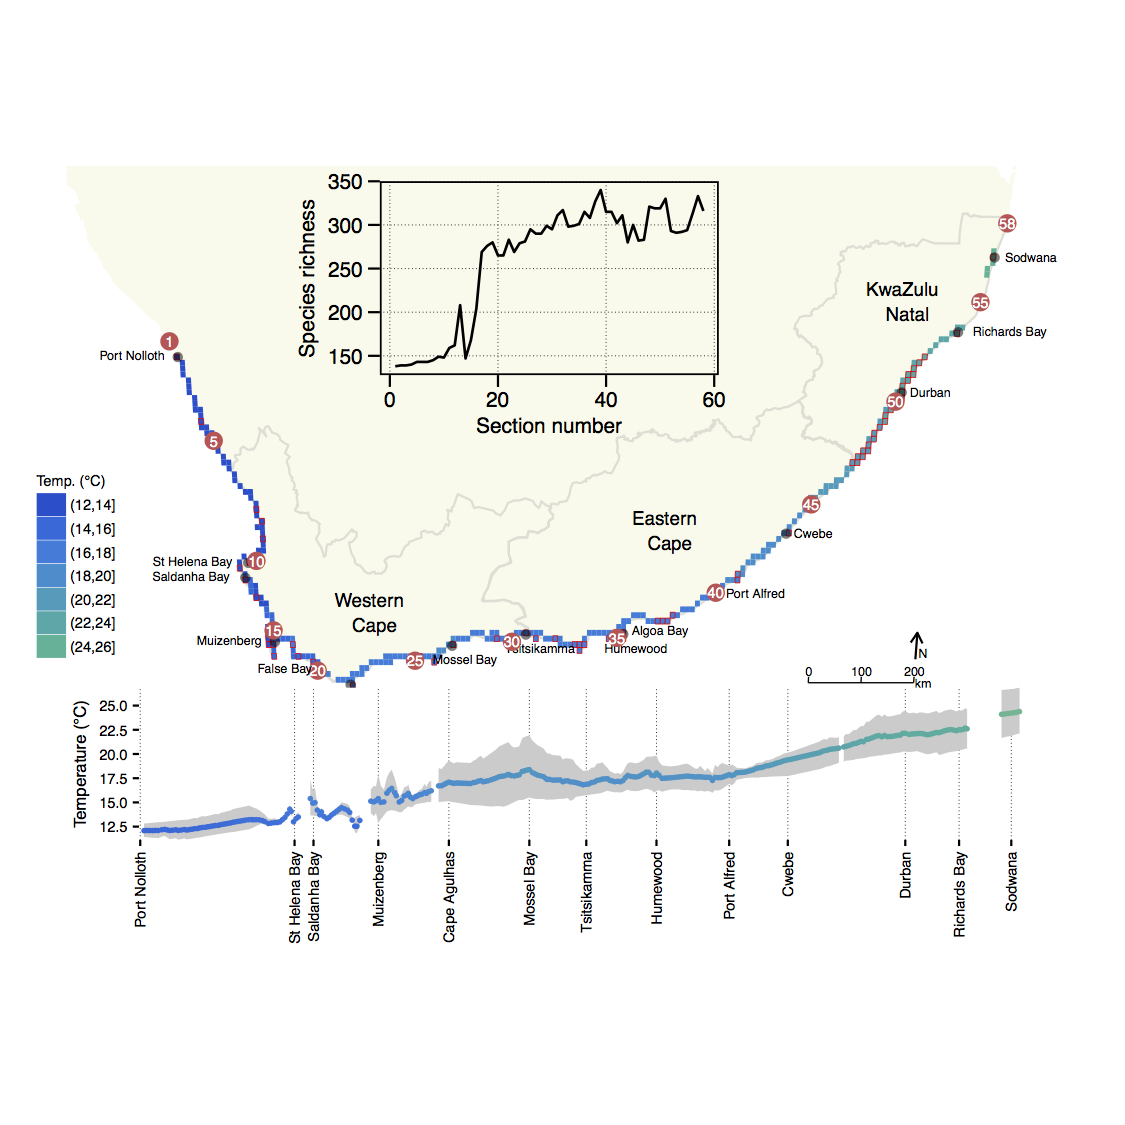
\includegraphics[width=1.0\textwidth]{../figures/Fig1.jpg}
\caption{{\bf Profile of mean annual temperature along the coast of South Africa.} Profiles are indicated as a function of geographical position on a coastal map (top) and as a function of distance away from Section \textbf{1} (bottom). The latter visualisation also indicates the long-term minimum (mean August) and maximum (mean February) temperatures as a grey shaded area around the annual mean temperature. The inset shows the species richness of macroalgae along the coast. Note that although a detailed temperature profile is displayed here, further analyses in this paper proceed with temperature data interpolated to the 58 sections for which seaweed diversity data are available.}
\label{fig1}
\end{figure}

\begin{figure}[!ht]
\centering
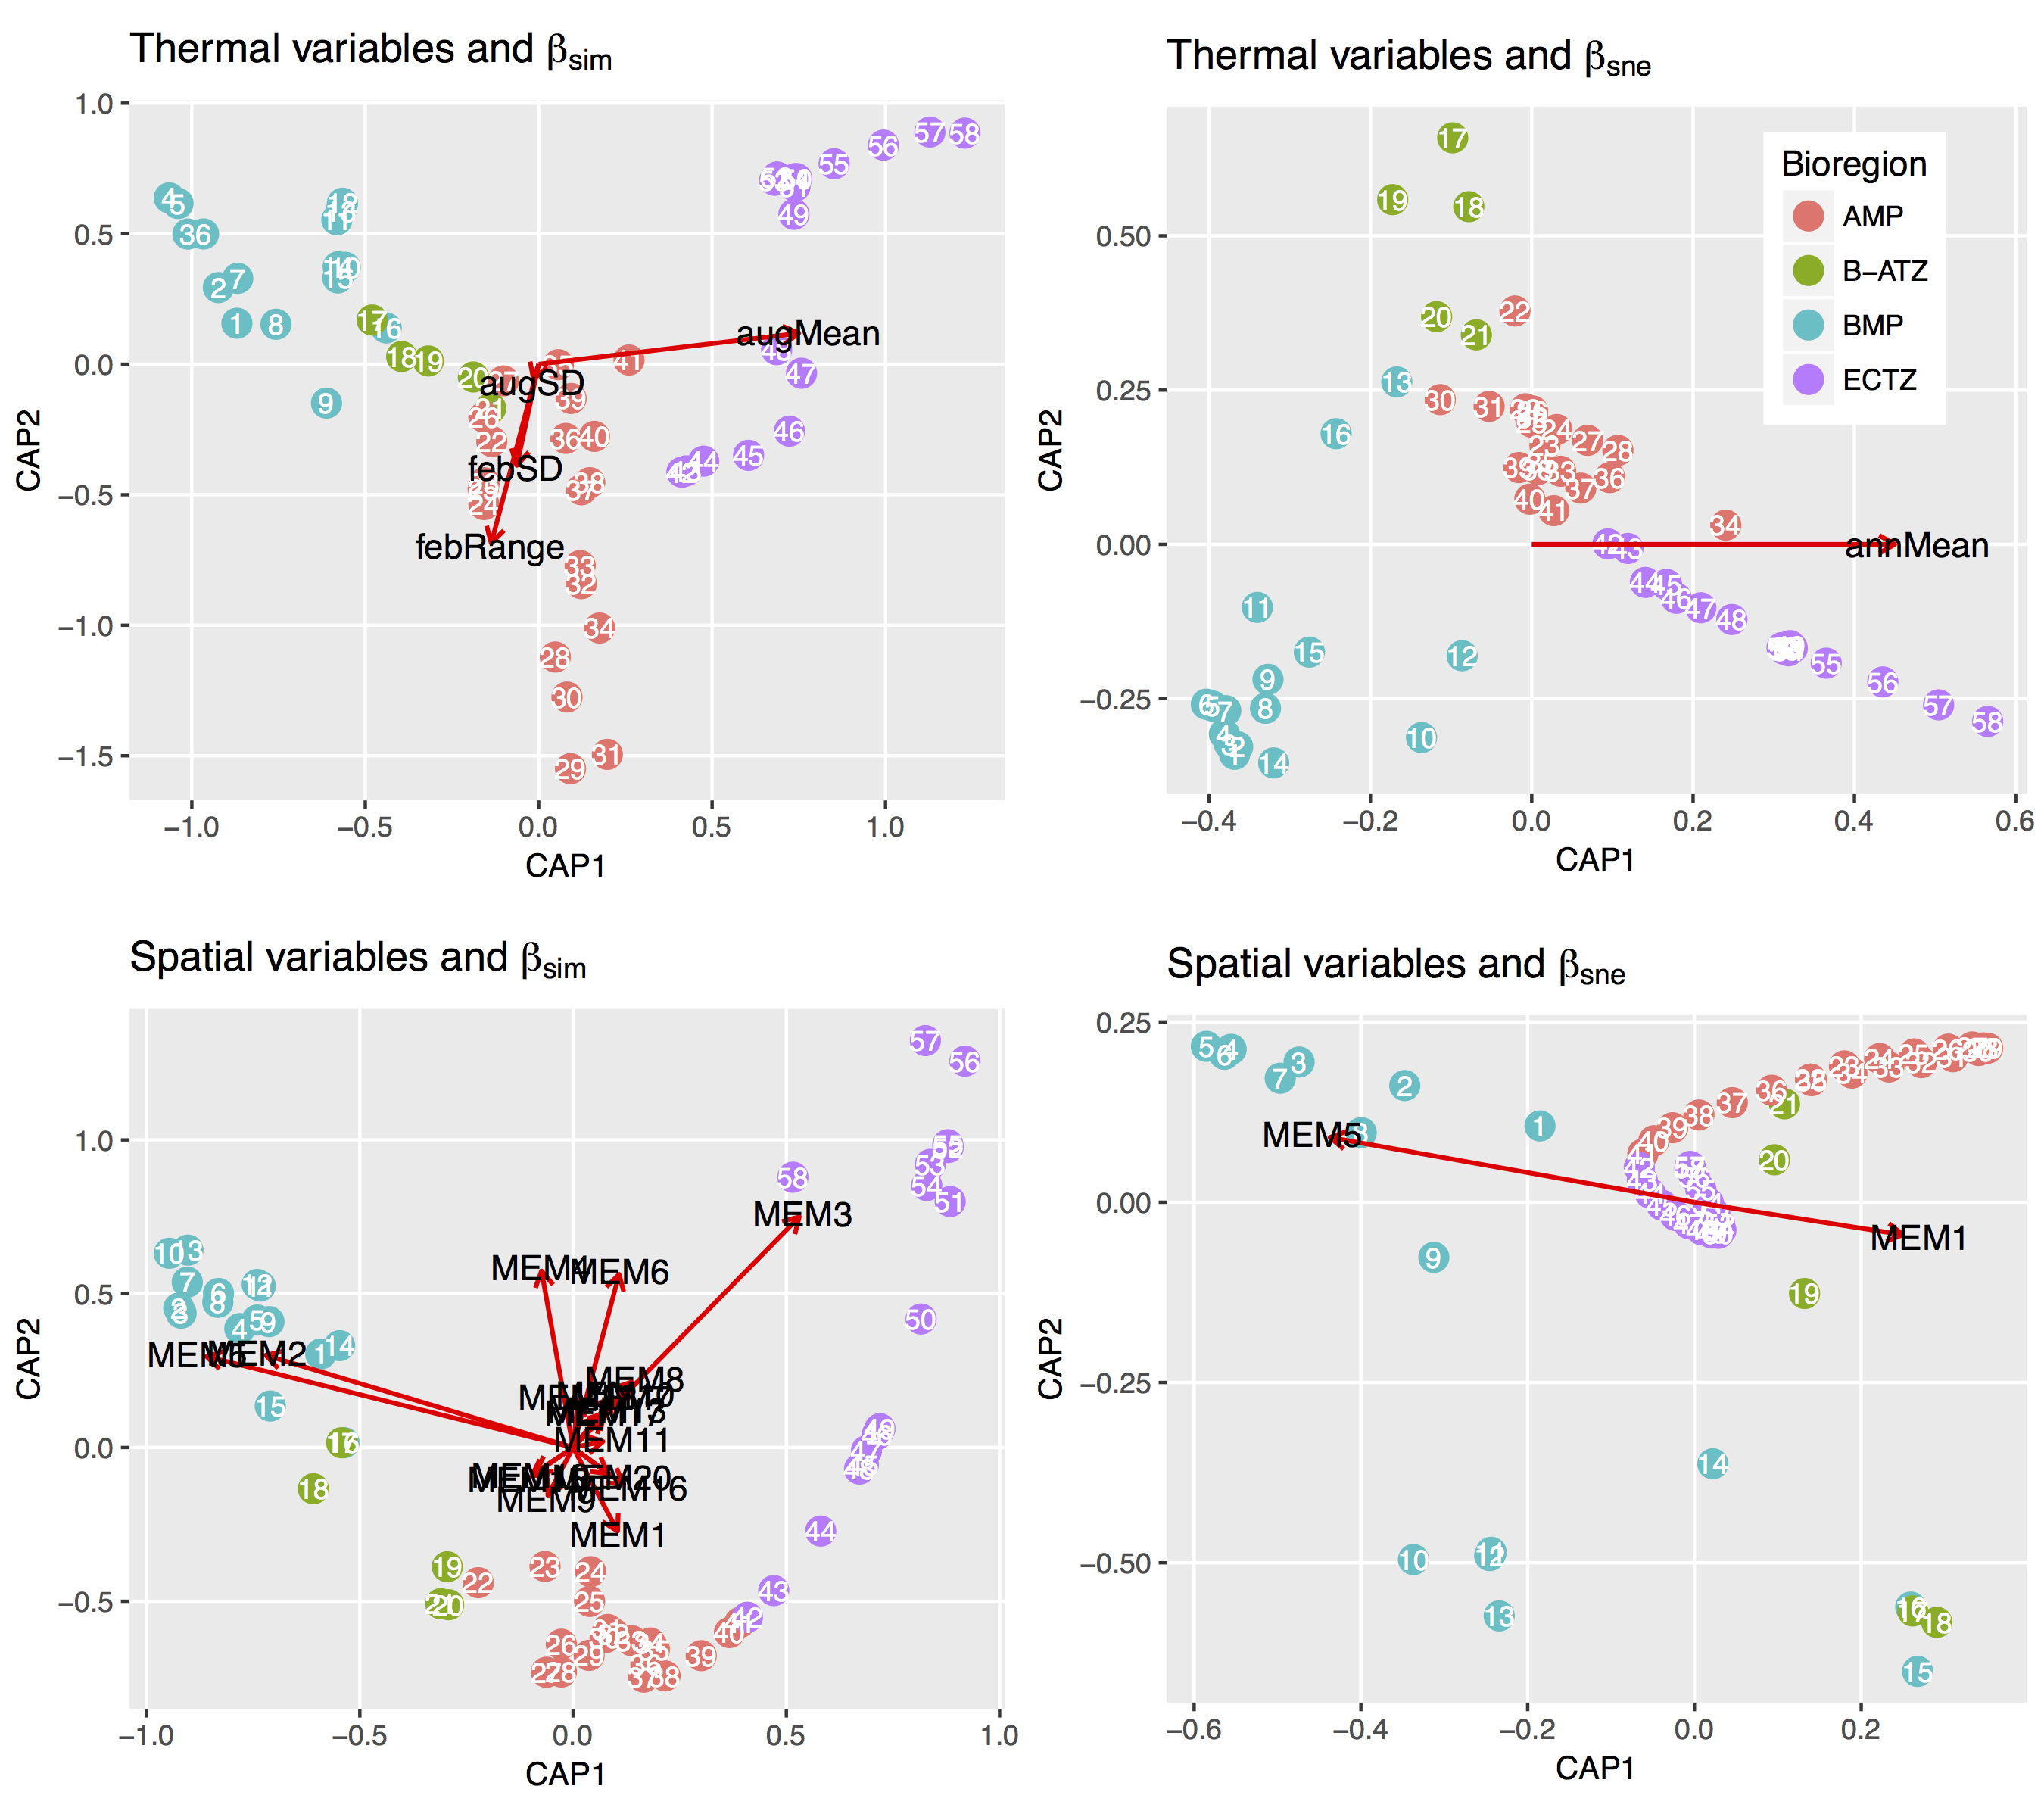
\includegraphics[width=1.0\textwidth]{../figures/Fig2.jpg}
\caption{{\bf db-RDA biplots of \texttt{lc} scores for \textbeta$_{\text{sim}}$ and \textbeta$_{\text{sne}}$ constrained by the thermal and spatial MEM variables.} The only two canonical axes shown are CAP1 and CAP2 since these capture the bulk of the inertia present in the ordinations. The constraining vectors were selected during the db-RDA steps.}
\label{fig2}
\end{figure}

\begin{figure}[!ht]
\centering
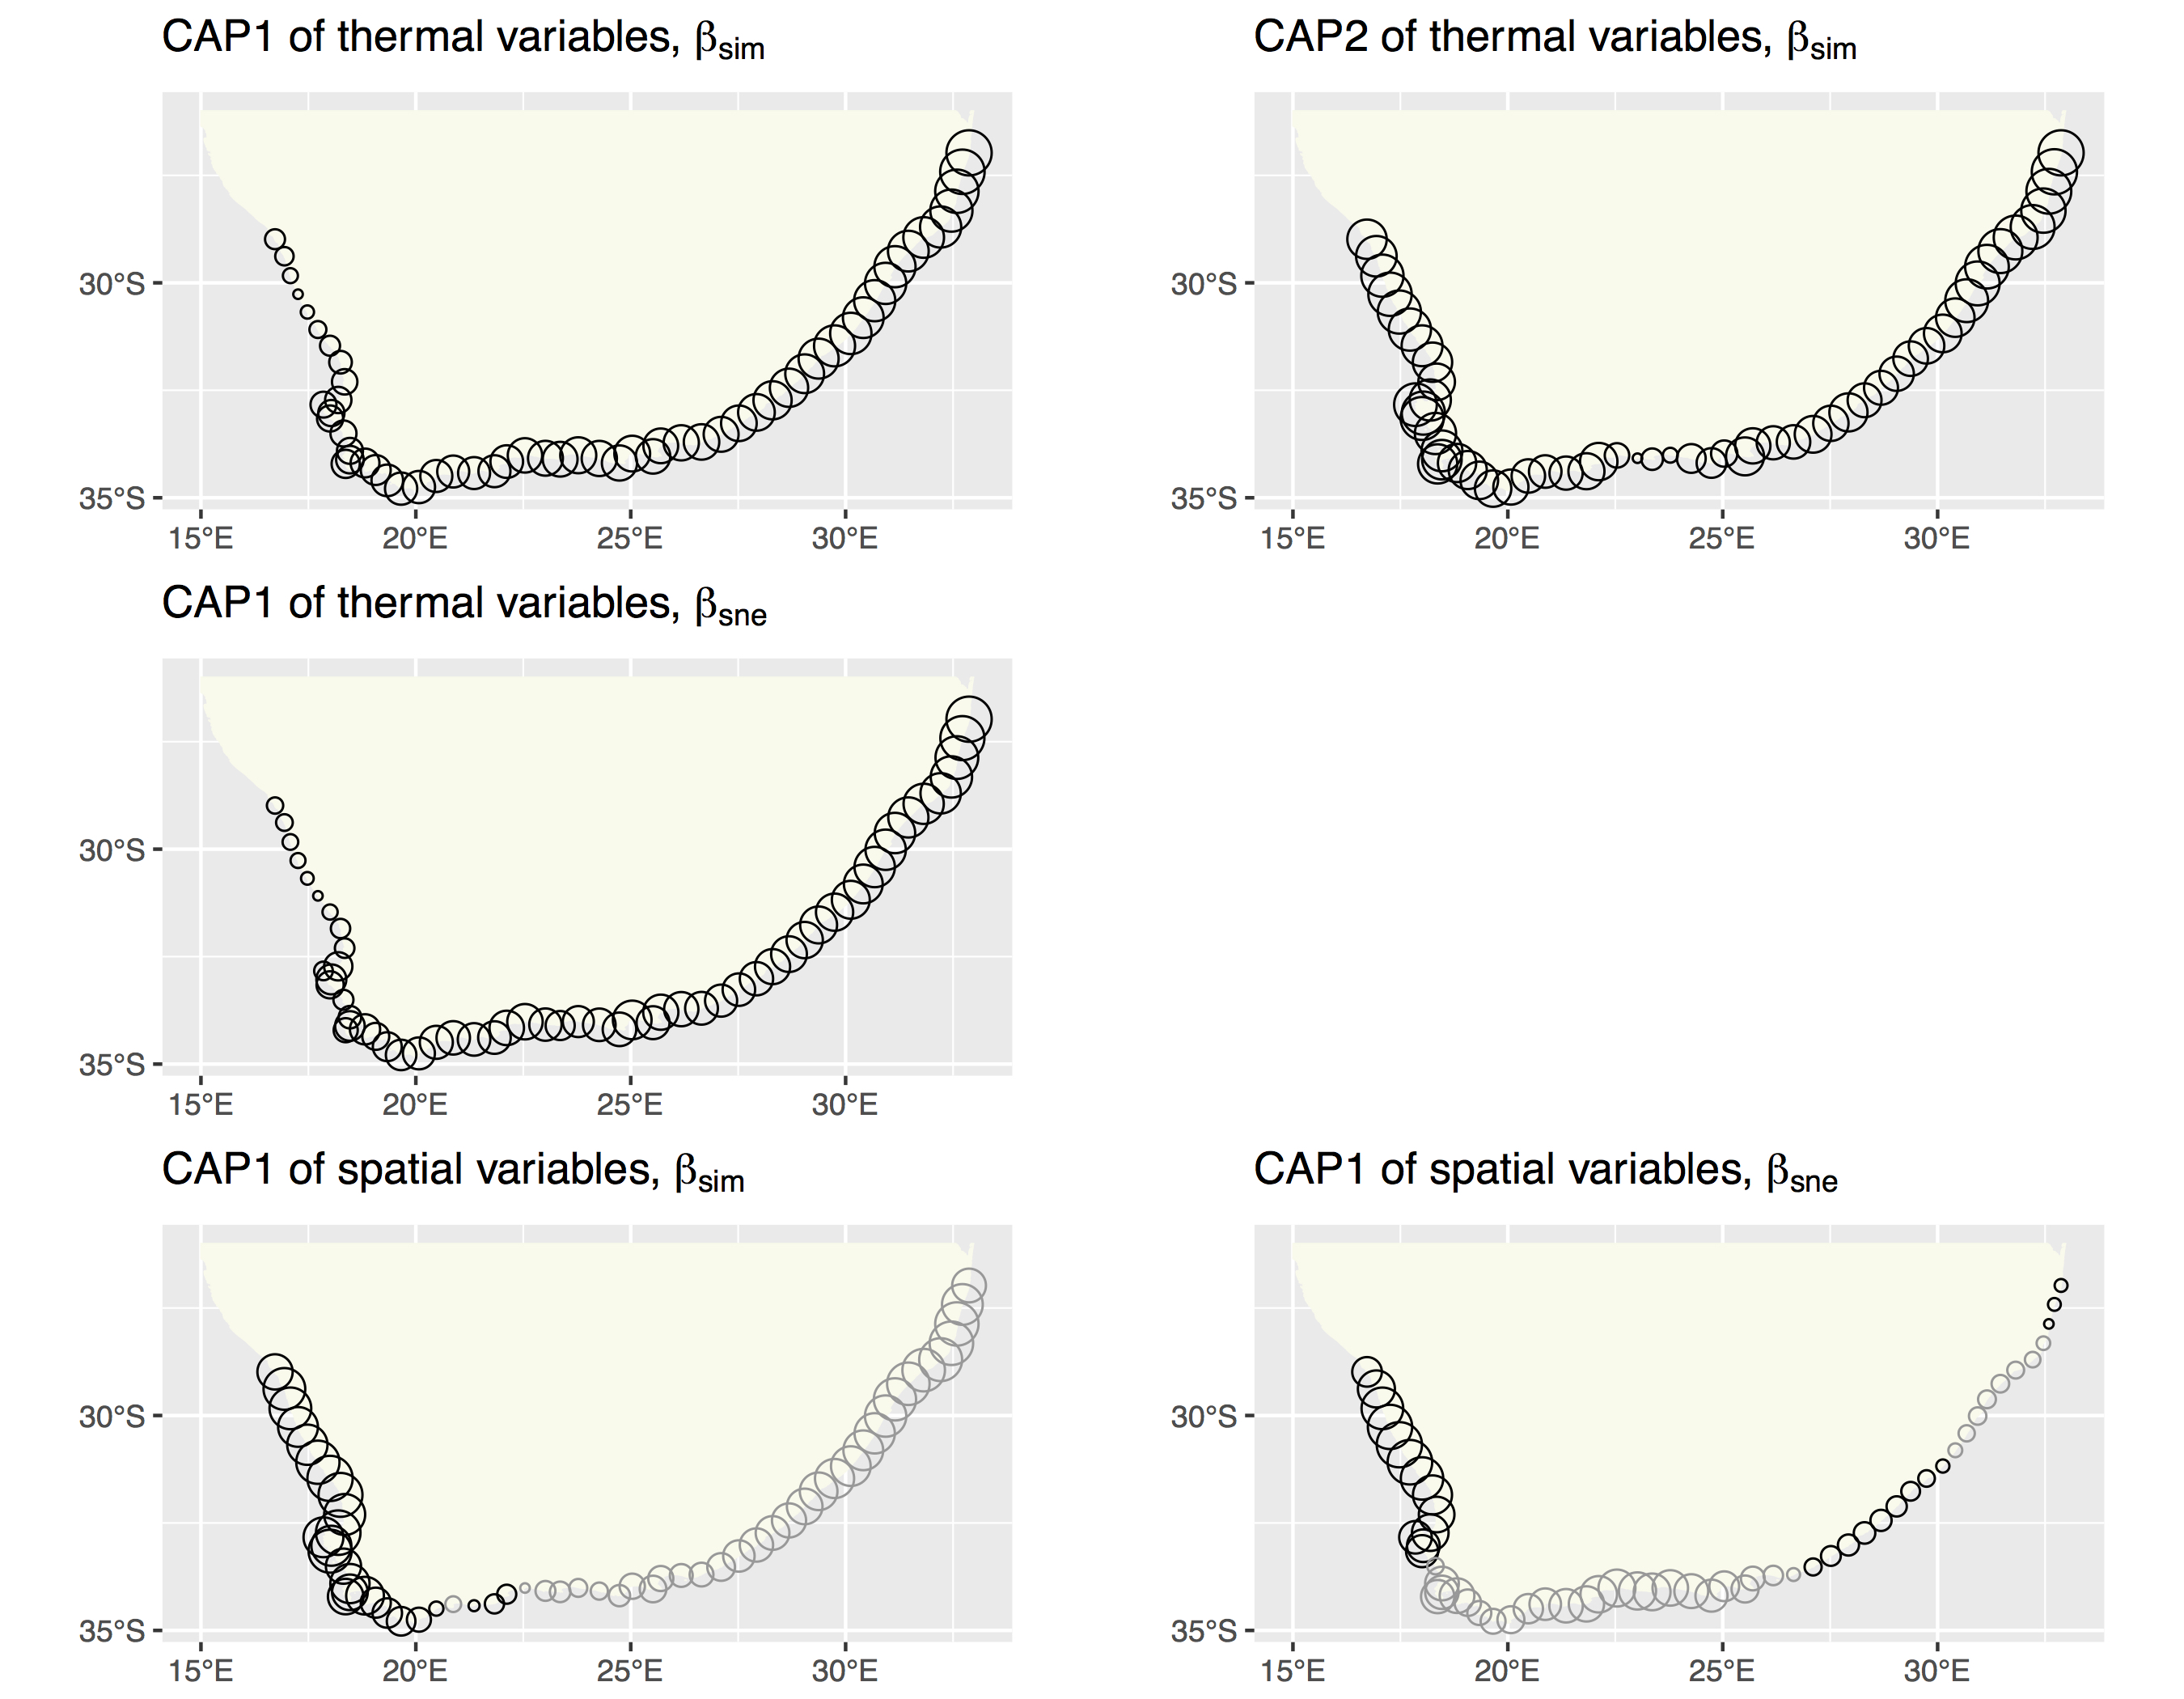
\includegraphics[width=1.0\textwidth]{../figures/Fig3.jpg}
\caption{{\bf db-RDA site scores for \textbeta$_{\text{sim}}$ and \textbeta$_{\text{sne}}$ on geographic coordinates.} The site scores indicate the major gradients captured by the environmental and spatial (MEM) constraints. Gray circles indicate negative site scores.}
\label{fig3}
\end{figure}

\begin{figure}[!ht]
\centering
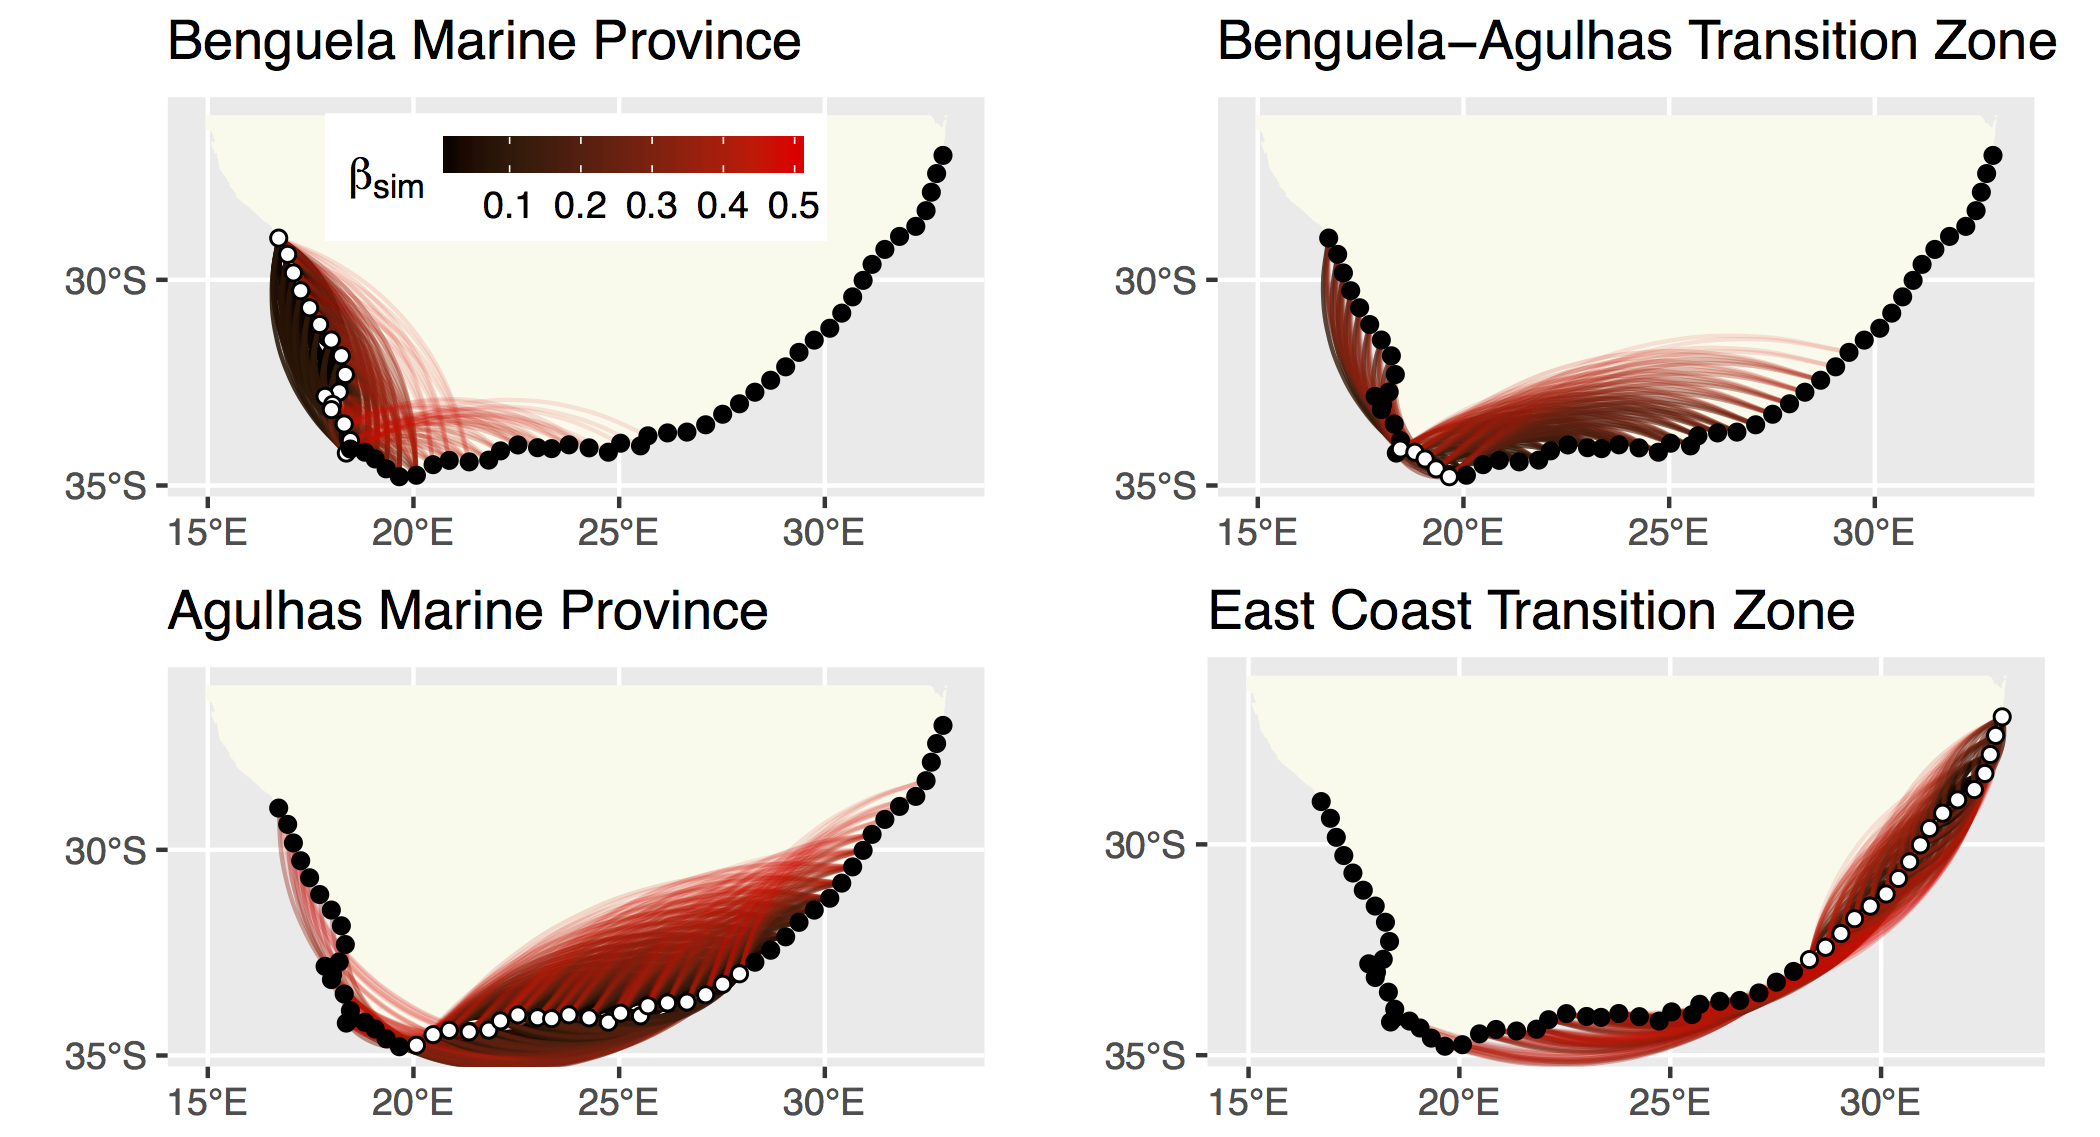
\includegraphics[width=1.0\textwidth]{../figures/Fig4.jpg}
\caption{{\bf Network graphs of pairwise \textbeta$_{\text{sim}}$ showing sections that are similar to one-another in species composition.} Dissimilarity indices range from \textgreater{}0.0--0.5 (possible dissimilarities range from 0.0--1.0). The 58 sections in Appendix A appear as dots at the vertices of the network graph, with those belonging with the `active' bioregion shown in white. The pairwise dissimilarities are shown by the coloured lines, with blacker lines indicating lower dissimilarity indices (species composition more similar) and redder ones higher dissimilarity indices (species composition more dissimilar).}
\label{fig4}
\end{figure}

\begin{figure}[!ht]
\centering
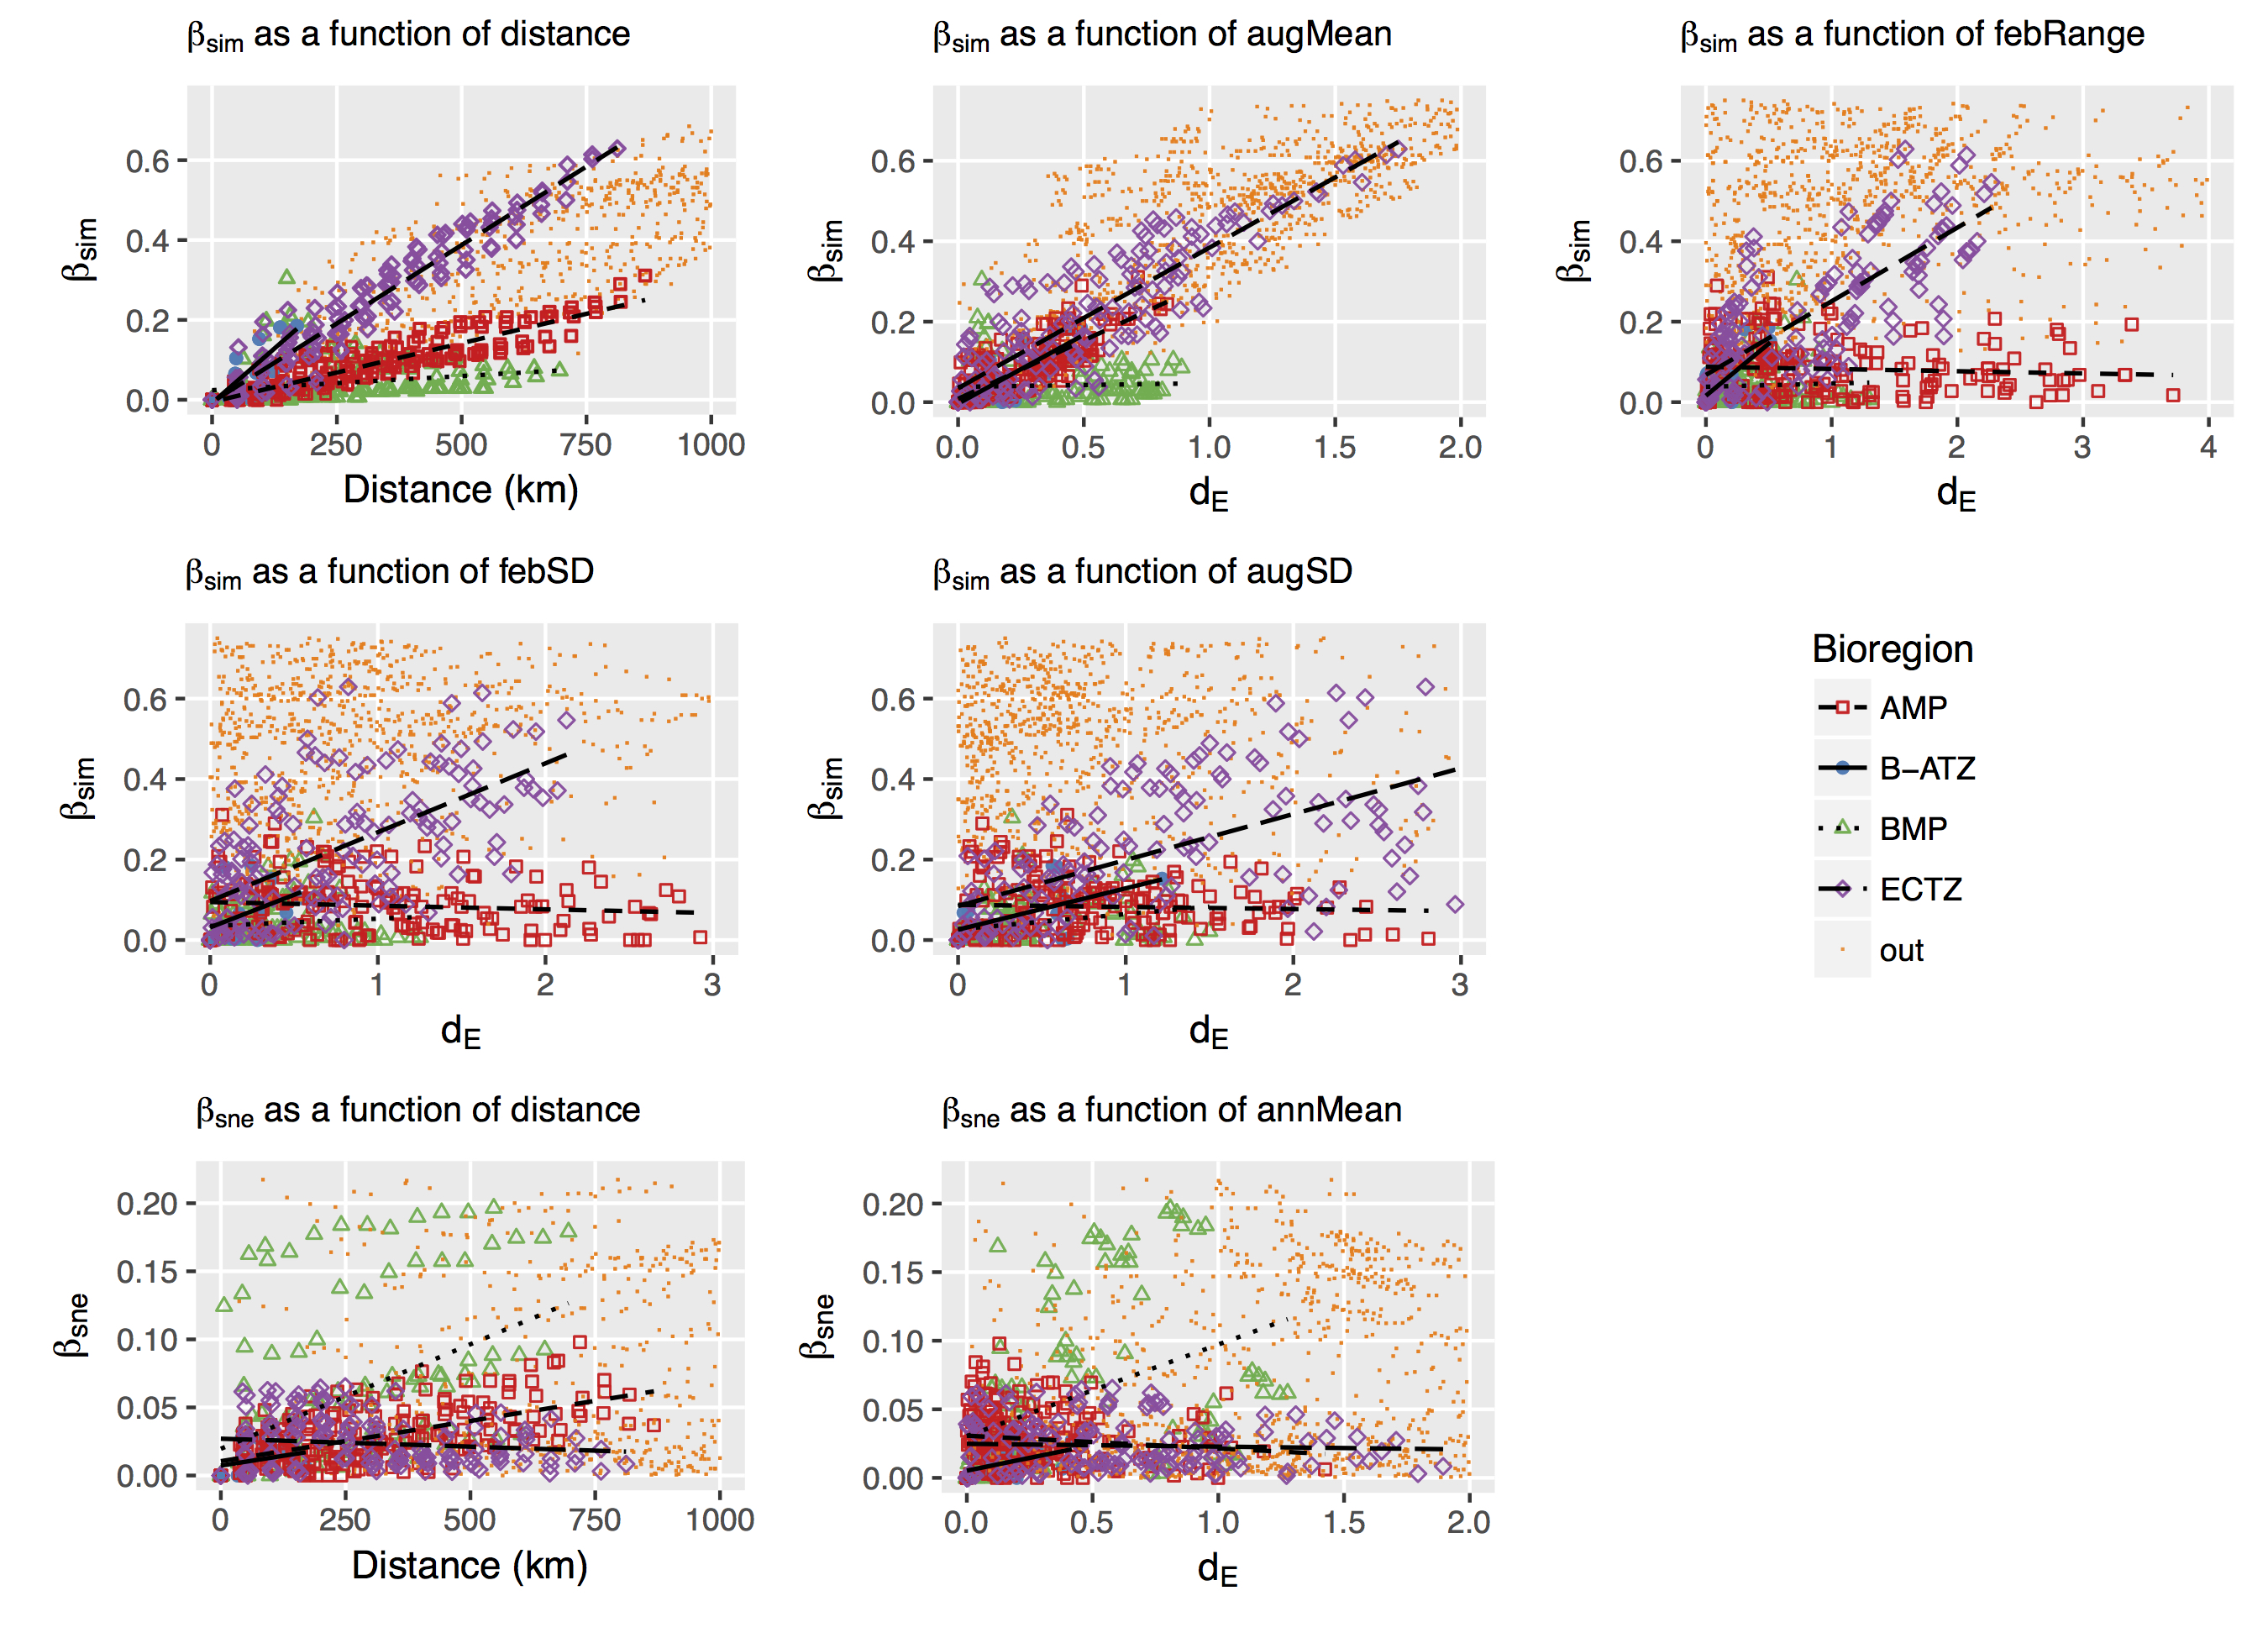
\includegraphics[width=1.0\textwidth]{../figures/Fig5.jpg}
\caption{{\bf Plots of the turnover (\textbeta$_{\text{sim}}$) and nestedness-resultant (\textbeta$_{\text{sne}}$) forms of \textbeta-diversity as a function of geographical or thermal distance between the coastal sections.} The influential d$_{\text{E}}$ variables (\emph{augMean}, \emph{febRange}, \emph{febSD} and \emph{augSD} for \textbeta$_{\text{sim}}$, and \emph{annMean} for \textbeta$_{\text{sne}}$) were determined in the db-RDA procedure.  \textbeta$_{\text{sim}}$, \textbeta$_{\text{sne}}$, d$_{\text{E}}$ and geographical distance were calculated as differences between coastal section pairs, and data points representing section pairs falling between bioregions are coloured yellow and labelled `out'. The strengths and gradients of the regression lines indicated in the panels are presented in Table~\ref{table3}.}
\label{fig5}
\end{figure}

%%% If you don't add the figures in the LaTeX files, please upload them when submitting the article.

%%% Frontiers will add the figures at the end of the provisional pdf automatically %%%

%%% The use of LaTeX coding to draw Diagrams/Figures/Structures should be avoided. They should be external callouts including graphics.

\end{document}
